
\documentclass{article}
\PassOptionsToPackage{numbers, compress}{natbib}
% Recommended, but optional, packages for figures and better typesetting:
\usepackage{microtype}
\usepackage{graphicx}
\usepackage{subcaption}
\usepackage{wrapfig}

\usepackage{hyperref}




\usepackage{caption}
% ===== preamble =====
\usepackage{booktabs} % for professional tables
\usepackage{multirow}
\usepackage[table]{xcolor}
\usepackage{tikz}
\usepackage{setspace}
% node for gap cells
\newcommand{\gapnode}[2]{%
  \tikz[remember picture,baseline=(#1.base)]%
    \node[inner sep=0pt,outer sep=0pt] (#1) {\makebox[2.4em][c]{\strut #2}};%
}

\usepackage{arydshln} % 必须放在 xcolor 之后

%\providecommand{\theHalgorithm}{\arabic{algorithm}}
% Attempt to make hyperref and algorithmic work together better:
%\newcommand{\theHalgorithm}{\arabic{algorithm}}
\providecommand{\theHalgorithm}{\arabic{algorithm}}


% Use the following line for the initial blind version submitted for review:
\usepackage[preprint]{neurips_2026}

\usepackage{amsmath}
\usepackage{amssymb}
\usepackage{mathtools}
\usepackage{amsthm}
% \usepackage{algorithm}
% \usepackage{algpseudocode}
% if you use cleveref..
\usepackage[capitalize,noabbrev]{cleveref}
% \usepackage{algorithm}
% \usepackage{algpseudocode}
%%%%%%%%%%%%%%%%%%%%%%%%%%%%%%%%
% THEOREMS
%%%%%%%%%%%%%%%%%%%%%%%%%%%%%%%%
\theoremstyle{plain}
\newtheorem{theorem}{Theorem}[section]
\newtheorem{proposition}[theorem]{Proposition}
\newtheorem{lemma}[theorem]{Lemma}
\newtheorem{corollary}[theorem]{Corollary}
\theoremstyle{definition}
\newtheorem{definition}[theorem]{Definition}
\newtheorem{assumption}[theorem]{Assumption}
\theoremstyle{remark}
\newtheorem{remark}[theorem]{Remark}

% Todonotes is useful during development; simply uncomment the next line
%    and comment out the line below the next line to turn off comments
%\usepackage[disable,textsize=tiny]{todonotes}
% \usepackage[disable]{todonotes}% todonotes

\usepackage[most]{tcolorbox}
\usepackage[normalem]{ulem}
\newcommand{\revdel}[1]{\textcolor{red}{\sout{#1}}}
\newcommand{\revadd}[1]{\textcolor{blue}{\uline{#1}}}

\newtcolorbox{fullwidthprompt}{
  width=\textwidth,
  colback=gray!5,
  colframe=black!50,
  boxrule=0.5pt
}

% The \icmltitle you define below is probably too long as a header.
% Therefore, a short form for the running title is supplied here:


\title{Toward Robust GraphRAG: Mitigating Retrieval Drift and Hallucination from Imperfect Knowledge Graphs}

\author{
  \textbf{Yizhuo Ma} \quad
  \textbf{Jinchuan Xu} \quad
  \textbf{Tao Wen} \quad
  \textbf{Qizhi Chen} \quad
  \textbf{Jiakai Li} \\
  \textbf{Rongzheng Wang} \quad
  \textbf{Muquan Li} \quad
  \textbf{Shuang Liang} \quad
  \textbf{Ke Qin} \\
  University of Electronic Science and Technology of China
}

\begin{document}

\maketitle

\begin{abstract}
%图检索增强生成依赖知识图作为结构检索索引来改进多跳推理并取得了不错的进展。然而现有的GraphRAG方法通常依赖大语言模型自动构建图谱，忽略了其中广泛存在的issue 模式，即虚假噪声和不完整信息。这些问题模式对多跳检索造成了两个挑战从而弱化了检索的鲁棒性，其中虚假噪声促使检索向结构合理但不受支持的证据漂移，而不完整的信息通过强制结构连续性引发检索幻觉。为了解决这些，我们提出了CS-RAG，这是一种用于在不完美知识图上进行鲁棒多跳检索的graphRAG框架。CS-RAG首先将每个查询规划为有序执行的的原子约束，并执行基于anchor和relation的细粒度检索，以防止检索的无约束扩展。然后，它应用充分性检查来决定检索到的证据是否可以安全地诱导变量绑定以进行后续传播从而抑制幻觉证据，并在结构支持不足时激活文本恢复。在多跳推理benchmarks上的的实验表明，CS-RAG在不同的知识图构建器上具有更强的鲁棒性，并且能在受控的杂散噪声和不完整信息注入下保持更稳定。


Graph Retrieval-Augmented Generation (GraphRAG) has become a common approach for multi-hop reasoning by using knowledge graphs (KGs) as structured retrieval indexes. However, most existing GraphRAG methods implicitly assume that LLM-constructed KGs provide structural support for evidence chaining. In this paper, we show that this assumption does not always hold in practice through an empirical analysis, and identify two recurring KG issue modes often overlooked by current retrievers: spurious noise and incomplete information. Spurious noise induces retrieval drift toward plausible but unsupported triples, whereas incomplete information leads to retrieval hallucination by forcing continuation through under-supported graph structure. To address these challenges, we propose CS-RAG, a robust GraphRAG framework that mitigates the impact of imperfect KGs during retrieval rather than relying on KG repair. CS-RAG first plans each query as an ordered sequence of executable atomic constraints and performs fine-grained anchor- and relation-aware retrieval to constrain evidence acquisition around the intended hop semantics. It then applies a sufficiency check to decide whether the retrieved evidence can safely induce variable bindings for subsequent propagation and activates textual recovery when structural support is insufficient, thereby reducing hallucinated structural continuation. Experiments on three multi-hop QA benchmarks show that CS-RAG is less sensitive to builder choice and remains stable under controlled KG issue injection.
Code is available at: \url{https://github.com/myz12138/CS-RAG/}
\end{abstract}


\section{Introduction}
\maketitle

\begingroup
\renewcommand{\thefootnote}{}
\footnotetext{
Emails: \texttt{myz@std.uestc.edu.cn}, \texttt{qinke@uestc.edu.cn}.

Corresponding author: Ke Qin. 
}
\endgroup

Retrieval-Augmented Generation (RAG)~\cite{rag1} grounds LLM~\cite{qwen3_technical_report_2025,meta2024llama33_modelcard,openai2025gpt5systemcard} outputs in external documents, but retrieval becomes brittle when a question requires several passages to be linked in a specific order. Graph Retrieval-Augmented Generation (GraphRAG)~\cite{graphrag_survey1,graphrag_survey2} addresses this limitation by using LLM-constructed knowledge graphs (KGs)~\cite{KG1,KG2,KG3} as structured retrieval indexes, making relations among evidence units explicit for multi-hop reasoning~\cite{rag_app2,RAG_APP1}. Recent methods exploit such graph structure through global propagation, learned graph scoring, or path-centric pruning to improve evidence expansion and selection, yielding promising results~\cite{hipporag,gfm-rag,pathrag,neuropath}.

\begin{figure*}[ht]
    \centering
    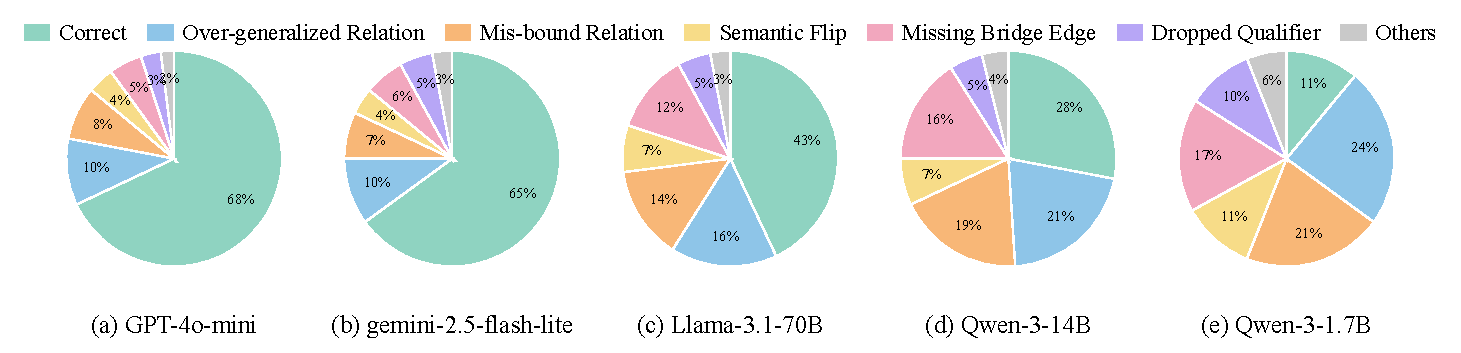
\includegraphics[width=0.98\linewidth]{Figs/observation_pie.pdf}
   \caption{Distribution of correct extractions and incorrect extraction patterns under different KG builders. The statistics are computed from sampled queries across MuSiQue, 2WikiMultihopQA, and HotpotQA, with 100 queries sampled from each dataset.}
    \label{fig:observation}
\end{figure*}

Despite their different retrieval designs, these methods largely share one implicit assumption that the constructed KG is reliable enough to serve as a structural index. 
However, this assumption can be fragile in practice because GraphRAG pipelines rely on LLM builders to construct KGs from source documents~\cite{builder1,builder2}, while deployment constraints such as privacy and cost may lead to different builder choices. These builders can differ substantially in parameter scale and extraction capability~\cite{builder3}, causing the resulting KGs to exhibit varying levels of quality issues that undermine downstream retrieval performance. As shown in Figure~\ref{fig:observation}, we observe the extraction quality of query-related gold supporting sentences across datasets under different KG builders. Extraction correctness is positively correlated with builder capability and model scale, yet even the strongest builder produces correct tuples for only 68\%.

In contrast, the remaining incorrect tuples are often overlooked during retrieval and can systematically distort hop-wise evidence acquisition once consumed as structural evidence. Specifically, we observe that these incorrect tuples fall into five recurring patterns, with low-frequency cases grouped as Others, and their proportions vary across builders. (Appendix~\ref{app:issue_patterns} provides detailed definitions of these patterns.) Based on their effects on downstream retrieval, we summarize these patterns into two broader issue modes: (1) \textbf{spurious noise}, including over-generalized relations, mis-bound relations, and semantic flips, and (2) \textbf{incomplete information}, including missing bridge edges and dropped qualifiers. The former preserves plausible graph connectivity but corrupts hop semantics, as fine-grained relations may be weakened into vague associations, attached to unsupported co-mentioned entities, or flipped in direction. The latter removes bridge edges or drops qualifiers such as time, location, and conditions, leaving the graph with incomplete structural support for multi-hop evidence chaining. This distinction gives rise to two retrieval challenges:

\begin{itemize}
\item \textbf{(1) Retrieval Drift.}
When the KG contains spurious noise, locally plausible but unsupported triples may still satisfy coarse relevance. Without enforcing the fine-grained constraints required by the current hop, retrieval can treat such triples as valid expansion points, inducing wrong bindings and drifting away from the intended evidence chain.

\item \textbf{(2) Retrieval Hallucination.}
When the KG contains incomplete information, the graph may not provide sufficient structural support for the current hop. Without verifying whether the retrieved candidates can safely support propagation, retrieval tends to continue through weak or partial evidence, producing unsupported bindings and hallucinated structural chains.
\end{itemize}

These challenges raise a key research question: \textit{how to achieve robust retrieval against KG issues?} Directly repairing the constructed KGs is intuitive but often impractical due to the substantial cost of re-extraction, verification, or manual correction. We therefore focus on mitigating the impact of KG issues during retrieval. To this end, we propose \textbf{CS-RAG} (\underline{C}onstraint-based and \underline{S}ufficiency-guided \underline{R}etrieval \underline{A}ugmented \underline{G}eneration), a robust framework for multi-hop retrieval over imperfect KGs. CS-RAG consists of two tightly coupled components for hop-wise evidence acquisition and propagation. \textbf{First}, it introduces a novel atomic-constraint planning scheme that maps a complex query into atomic constraints with explicit intermediate variables and relation variants (e.g., \textit{Apollo 13} -- \{\textit{nominated for}, \ldots, \textit{up for}\} -- ?award). Retrieval is then executed around these constraint-level semantics, reducing coarse query matching and filtering out loosely relevant but spurious triples. \textbf{Second}, We introduce a hop-wise sufficiency criterion into multi-hop retrieval for the first time, and prove that it yields a lower bound on the top-candidate probability, thereby providing a principled way to block ambiguous bindings before they propagate into hallucinated chains. Specifically, CS-RAG performs a distribution-based check to decide whether the retrieved candidates provide reliable support for structural binding or whether textual recovery should instead be triggered. Our contributions are as follows:

1. We empirically show that the common reliable-KG assumption in GraphRAG does not always hold, and reveal that query-relevant incorrect tuples concentrate around recurring extraction patterns that can be summarized into two issue modes: spurious noise and incomplete information.

2. We propose CS-RAG, a robust GraphRAG framework over imperfect KGs. CS-RAG introduces atomic constraints with explicit intermediate variables and relation variants to constrain evidence acquisition against retrieval drift, and further incorporates a distribution-based sufficiency check into hop-wise propagation for the first time to reduce hallucinated structural continuation.

3. Experiments on three multi-hop QA benchmarks show that CS-RAG achieves stronger robustness under both cross-builder evaluation and controlled KG issue injection.


\section{Related Work}

\subsection{Graph-structured Retrieval}
Early graph-structured retrievers such as GraphRAG~\cite{graphrag1} and HippoRAG~\cite{hipporag} propagate query relevance over a graph index via global community detection or Personalized PageRank~\cite{page1999pagerank}. Follow-up systems combine unstructured vector search with structured neighborhood expansion to cover dispersed evidence~\cite{lightrag}. More recent learned retrievers, including GNN-RAG~\cite{GNN-RAG}, G-Retriever~\cite{G-retrieval}, and SubgraphRAG~\cite{subgraphrag}, use graph neural networks to score nodes or subgraphs with learned structural features, while graph foundation models explore zero-shot retrieval across graph domains~\cite{gfm-rag}. However, these methods generally treat the constructed KG as a dependable retrieval index, and thus do not explicitly guard hop-wise retrieval against builder-induced spurious noise. As a result, structurally plausible but unsupported triples can be amplified during graph matching or propagation, leading to retrieval drift under imperfect KGs.

\subsection{Iterative Multi-hop Retrieval}
To manage retrieval complexity, this line of work refines the search space through iterative selection and controlled expansion. Methods such as ToG~\cite{tog}, ToG2~\cite{tog2}, KAG~\cite{kag}, and PathRAG~\cite{pathrag} formulate retrieval as sequential path construction, using LLM-driven decisions or flow-based heuristics to prune branches and retain salient trajectories. Some variants further incorporate symbolic query solvers or schema-guided planning to align intermediate steps with graph structure~\cite{youturag}. Similarly, NeuroPath~\cite{neuropath} and HippoRAG~\cite{hipporag} restrict the retrieval scope based on intermediate generations, using partial outputs to steer later queries. To control computational costs, flow-based allocation and adaptive expansion thresholds balance search breadth and depth~\cite{pathrag}. However, these methods usually assume each step can continue through available graph structure without verifying whether current evidence is sufficient, which may force retrieval along weak connections when bridge edges or qualifiers are missing and cause retrieval hallucination under incomplete KGs.

% =========================
%  CS-RAG Method (Challenge 1 Part Only)
%  Save as: method_challenge1.tex
% =========================

% =========================
%  CS-RAG Method (Challenge 1 Part Only, Revised)
%  Save as: method_challenge1.tex
% =========================
% \section{Motivating Observations}
% \label{sec:observations}

% To strengthen constraint-grounded retrieval and prevent noise propagation, we inspect representative failure cases of GraphRAG baselines and analyze their retrieval traces to identify the concrete causes of multi-hop breakdown.



% % -----------------------------
% % Observation 1
% % -----------------------------
% \subsection{Observation I: Missing-Evidence Types in Failed Retrieval}
% \label{sec:obs1}

% We analyze retrieval failures from several representative GraphRAG baselines, including HippoRAG and GNN-RAG that perform single-pass retrieval without query decomposition,
% and a decomposition-based baseline (denoted as \textsc{DecompBaseline}) that retrieves evidence step-by-step.
% For each baseline, we randomly sample 100 failed examples, where the final answers are incorrect and the failure can be attributed to incomplete evidence retrieval.

% For each failed example within single-pass retrieval, we categorize the missing evidence types and summarize their distribution in Figure~\ref{fig:obs_failure_modes}.
% Concretely, we distinguish whether the missing evidence corresponds to \textbf{explicit} signals that are directly expressed on the query surface
% (e.g., salient anchor entities or surface relations), or \textbf{implicit} signals that are not explicitly stated but are required to bridge reasoning hops
% (e.g., hidden relations or bridge entities).

% We find that, for single-pass baselines, the majority of failures are not due to losing explicit anchors or surface relations:
% the retriever can largely recover query-mentioned anchors and surface cues (\xx\% of the sampled failures fall into the explicit-covered category).
% Instead, their dominant failure source is missing implicit hop-bridging evidence, i.e., the retriever fails to retrieve the hidden relations or intermediate entities
% needed to connect evidence across hops.

% We further examine failures of the decomposition-based baseline and observe that a substantial fraction of its failures (\xx\%) are caused by semantic-near relation mismatch, where the retrieved relations are near-synonymous or loosely related to the intended constraint but do not support the correct reasoning transition. This indicates that, although stepwise decomposition can partially expose implicit constraints, the retrieved relation coverage may still be unstable when fine-grained constraints are not enforced.

% These analyses suggest that retrieval patterns lacking fine-grained constraint grounding tend to produce evidence chains that are surface-aligned yet hop-incomplete,
% or drift to semantically plausible but logically incompatible transitions, thereby undermining multi-hop reasoning reliability.

% \begin{figure}[t]
%     \centering
%     \includegraphics[width=0.85\linewidth]{figs/obs_failure_modes.pdf}
%     \caption{Distribution of missing-evidence types on 100 randomly sampled failures per baseline.
%     Single-pass baselines (e.g., HippoRAG, GNN-RAG) mainly fail due to missing implicit hop-bridging evidence,
%     while decomposition-based retrieval shifts failures toward semantic-near but incorrect relation coverage.}
%     \label{fig:obs_failure_modes}
% \end{figure}


% % -----------------------------
% % Observation 2
% % -----------------------------
% \subsection{Observation II: Candidate Score Distributions Signal Solvability}
% \label{sec:obs2}

% We further investigate whether the shape} of the candidate score distribution can indicate whether a retrieval step is reliable.
% For each retrieval step, a baseline returns a top-$K$ candidate set with a normalized score/top-probability distribution.
% We divide retrieval steps into two groups:
% \textbf{Correct steps}, where the candidate set contains a gold supporting tuple (or evidence unit), and
% \textbf{Incorrect steps}, where none of the candidates correspond to gold support.

% Figure~\ref{fig:obs_score_distribution} compares the candidate distribution statistics between correct and incorrect steps.
% We find that correct steps typically produce peaked} distributions where a few candidates dominate the probability weight,
% while incorrect steps exhibit flat} distributions with high uncertainty, indicating that the retriever cannot confidently distinguish correct evidence.
% This distributional signature implies that uncertainty-aware filtering is necessary to prevent unreliable steps from propagating errors across hops.

% \begin{figure}[t]
%     \centering
%     % Replace with your generated plot (histogram / density plot).
%     \includegraphics[width=0.85\linewidth]{figs/obs_score_distribution.pdf}
%     \caption{Candidate distribution comparison between correct and incorrect retrieval steps.
%     Correct steps exhibit peaked distributions (high confidence), while incorrect steps are flatter (high uncertainty), suggesting that uncertainty-aware control is needed to avoid cascading errors.}
%     \label{fig:obs_score_distribution}
% \end{figure}



\section{Methodology}
\subsection{Overview}
Figure~\ref{fig:framework} illustrates the workflow of CS-RAG. Given a query and a constructed KG, CS-RAG first builds an ordered constraint plan with explicit relation semantics and intermediate variables, and then performs constraint-based retrieval for executable constraints. After that, it uses sufficiency-guided propagation and recovery to decide whether resolved bindings should ground later constraints or unresolved hops should trigger textual recovery. The resulting evidence is packed into constraint-aligned context for LLM generation.

\begin{figure*}
    \centering
    
\includegraphics[width=0.97\linewidth]{Figs/framework.pdf} 
    \caption{The Overview of CS-RAG's workflow.}
    \label{fig:framework}
\end{figure*}

\subsection{Constraint-based Retrieval}
We first convert a multi-hop query into an ordered constraint plan with variables and relation variants, and retrieve structural candidates in a constraint-based manner.
Each constraint is grounded by anchoring on observed entities, restricting the search to a localized one-hop neighborhood, and reranking candidates with relation-level and contextual signals.

\paragraph{Atomic Constraint Planning.}
Given a query $q$, we use a LLM-based planner to produce a structured plan
$\mathcal{P}=\langle \tau_1,\tau_2,\ldots,\tau_k\rangle$,
where each atomic constraint is represented as a triple pattern
$\tau_i=(h_i,r_i,t_i)$.
The head and tail are drawn from a unified symbol space consisting of constant entities extracted from $q$ and at least one unknown variable.
We denote the entity set by $\mathcal{E}_q$ and the variable set by $\mathcal{V}=\{?v_1,?v_2,\ldots\}$. Each variable is defined with a “\textit{?}” placeholder and a type specification, which denote an intermediate entity slot and potentially shared across multiple constraints.

For each $\tau_i$, the planner also generates a set of $m$ relation variants
$\mathcal{R}_i=\{r_i^{(1)},\ldots,r_i^{(m)}\}$.
This set makes the intended relational semantics explicit by enumerating plausible relation expressions implied by the query, and it provides an alignment target for later retrieval.
During constraint-based retrieval, we use $\mathcal{R}_i$ to match and filter KG relations at a finer granularity.

\paragraph{Anchor Matching.}
We first focus on atomic constraints that contain a single unknown variable, since such constraints can be grounded by at least one observed constant entity.
We define these atomic constraints as
\begin{equation}
\mathcal{P}_1 = \{\tau_i=(h_i,r_i,t_i)\in\mathcal{P}\mid |\{h_i,t_i\}\cap\mathcal{V}|=1\}.
\end{equation}
For each $\tau_i\in\mathcal{P}_1$, we denote the constant endpoint as the anchor surface form $e_i^{surf}\in\mathcal{E}_q$,
and treat the other endpoint as the unique variable whose assignment will be induced by retrieval.

Let the constructed KG be $\mathcal{G}=(\mathcal{E},\mathcal{R},\mathcal{T})$,
where $\mathcal{T}\subseteq\mathcal{E}\times\mathcal{R}\times\mathcal{E}$ is the triple set.
We map $e_i^{surf}$ to anchor nodes \(\mathcal{E}^{anchor}_i \subset \mathcal{E}\) using top-3 token-coverage matching between the query entity mention and KG entity names. 
Starting from $\mathcal{E}^{anchor}_i$, we enumerate the one-hop neighborhood to form the candidate pool $\mathcal{C}_i$.
This localized enumeration restricts retrieval to neighborhoods directly connected to the anchor, while preserving candidates that can instantiate the unique variable in $\tau_i$.

\paragraph{Relation Alignment and Contextual Reranking.}
For each candidate triple $c\in\mathcal{C}_i$ associated with $\tau_i$,
we first compare its KG relation against the relation variants in $\mathcal{R}_i$ and retain the top-$R$ aligned candidates to obtain $\mathcal{C}_i^{init}$.
This step focuses retrieval on relations aligned with the intended constraint.
We then apply a cross-encoder reranker for contextual scoring.
For each $c\in\mathcal{C}_i^{init}$, we score the concatenated input of the query, the linearized constraint, and the linearized candidate triple, and keep the top-$K_s$ candidates as the refined pool $\mathcal{C}_i^{top}$.
This step yields a compact candidate pool that is aligned with the current atomic constraint, avoiding selections that are merely semantically related but violate the intended relation.


\subsection{Sufficiency-Guided Propagation and Recovery}
This stage performs a sufficiency check to decide whether to propagate structural bindings or trigger textual recovery.
A sufficiency signal is firstly computed to determine whether an atomic constraint can be grounded with adequate structural support.
Constraints that pass the check are integrated into stable variable bindings and used for subsequent propagation, while constraints that fail the check drop structural propagation and activate textual recovery.

\paragraph{Sufficiency Scoring.}
For each atomic constraint $\tau_i\in\mathcal{P}_1$, the previous step returns a refined candidate pool $\mathcal{C}_i^{top}$
with cross-encoder scores $\{z_{i,c}\}_{c\in\mathcal{C}_i^{top}}$.
We normalize these scores with softmax into a probability distribution $\{p_{i,c}\}$ over the candidates, and compute the effective number of candidates:
\begin{equation}
N_{\mathrm{eff}}(\tau_i)=\frac{1}{\sum_{c\in\mathcal{C}_i^{top}}p_{i,c}^2}.
\label{eq:neff}
\end{equation}
A smaller $N_{\mathrm{eff}}(\tau_i)$ indicates a concentrated distribution and a more sufficient match, while a larger value indicates ambiguity.
We use a threshold $\gamma$ to determine whether $\tau_i$ is sufficiently grounded by structural evidence. Appendix~\ref{app:neff} provides the theoretical justification for this criterion.
\begin{equation}
\mathrm{State}(\tau_i) =
\begin{cases}
\mathrm{Resolved},   & N_{\mathrm{eff}}(\tau_i) \le \gamma,\\
\mathrm{Unresolved}, & N_{\mathrm{eff}}(\tau_i) > \gamma.
\end{cases}
\label{eq:state}
\end{equation}
We denote the corresponding resolved and unresolved constraint sets by $\mathcal{P}_R$ and $\mathcal{P}_U$.


\paragraph{Textual Recovery for Unresolved Constraints.}
For an unresolved constraint $\tau_u\in\mathcal{P}_U$, we activate textual recovery to supplement evidence without committing uncertain structural bindings.
Given a query-specific set of passages $U(q)$, we first retrieve the top-$K_t'$ ($K_t'$=8) passages by measuring semantic similarity between the linearized constraint and each passage. 
We then rerank the retrieved passages with a cross-encoder over the query, the current constraint, and the passage text, and keep the top-$K_t$ passages as the supplemental textual evidence set $\mathcal{T}_u^{txt}$.
This recovery branch reduces propagating uncertain structural bindings.


\paragraph{Binding and Propagation for Resolved Constraints.}
Each resolved constraint $\tau_i\in\mathcal{P}_R$ contains exactly one variable $v$.
We extract its induced entity set $\mathcal{E}_i(v)$ from $\mathcal{C}_i^{top}$ by collecting the candidate entities at the variable endpoint of the refined triples.
When $v$ appears in multiple resolved constraints, we integrate their candidate sets by intersection to enforce consistency, and fall back to the union when the intersection is empty.
The resulting binding set is denoted by $\mathcal{E}_b(v)$.

The binding set $\mathcal{E}_b(v)$ provides a stabilized assignment for subsequent constraint grounding.
For each resolved constraint, we further update its structural pool to $\hat{\mathcal{C}}_i^{top}$ by retaining only candidates consistent with $\mathcal{E}_b(v)$.
After that, we collect textual evidence to provide grounded support for each resolved atomic constraint.
For each resolved constraint $\tau_i\in\mathcal{P}_R$, the evidence $\mathcal{T}_i^{txt}$ is obtained by collecting the source passages associated with the triples in the updated structural pool $\hat{\mathcal{C}}_i^{top}$.

We then propagate the bindings to constraints that contain two variables.
Let $\mathcal{P}_2$ denote the set of constraints in $\mathcal{P}$ whose head and tail are both variables.
For a two-variable constraint $\tau_j=(v_a,r_j,v_b)\in\mathcal{P}_2$, if one endpoint variable already has a binding set such as $\mathcal{E}_b(v_a)$,
we instantiate $v_a$ as an observed anchor, turning $\tau_j$ into a one-variable constraint with one grounded endpoint.
We then rerun the same pipeline from constraint-based retrieval to sufficiency check to induce candidates for $v_b$ and collect the corresponding evidence.
By performing this propagation procedure again, constraints that initially contain two variables can also be progressively grounded while preserving the same constraint-level control.


\subsection{LLM Generation}
Finally, we pack evidences into constraint-aligned blocks:
\begin{equation}
B_i=\big[\,\mathrm{Lin}(\tau_i),\ \mathcal{T}_i^{txt}\big],\qquad
\mathcal{B}_q=\{B_i\}_{i=1}^{k},
\label{eq:evidence_blocks}
\end{equation}
yielding an ordered evidence context aligned with atomic constraints.
The resulting context $\mathcal{B}_q$ is fed into the language model to produce the final answer for the multi-hop query.



\section{Experiments}

\paragraph{Datasets and Baselines.}
We evaluate CS-RAG on three standard multi-hop QA benchmarks: 2WikiMultihopQA~\cite{2wiki}, HotpotQA~\cite{hotpotqa}, and MuSiQue~\cite{Musique}.
Following HippoRAG~\cite{hipporag}, we use the same fixed subset of 1{,}000 validation instances adopted by prior work, and apply it consistently to all methods for fair comparison.
We compare CS-RAG with representative GraphRAG baselines, including LightRAG~\cite{lightrag}, HippoRAG2~\cite{hipporag2}, GFM-RAG~\cite{gfm-rag}, and NeuroPath~\cite{neuropath}. We evaluate all baselines using their released implementations and follow their official evaluation settings.
These baselines represent diverse ways of exploiting KG structure for downstream reasoning. 


\paragraph{Experimental Details.}
We use all-MiniLM-L6-v2~\cite{sentence-bert} as the dense retriever and bge-reranker-v2-m3~\cite{bge-reranker-v2-m3} as the cross-encoder reranker. GPT-4o-mini~\cite{gpt-4o} is used for atomic constraint planning and final answer generation. All experiments were run with Python 3.10 on an NVIDIA GeForce RTX 4090 server, with LLM-based KG construction, planning, and answer generation performed through API calls.
We evaluate downstream QA performance using Exact Match (EM) and token-level F1, and retrieval quality using Recall@5 over gold evidence. Additional implementation details are provided in Appendix~\ref{app:detail}.

% Required packages:
% \usepackage{booktabs}
% \usepackage[table]{xcolor}
% \usepackage{multirow}
% \usepackage{graphicx}

\definecolor{AvgColor}{HTML}{7B3294}
\definecolor{StdColor}{HTML}{008837}

\providecommand{\metric}[1]{\textsc{#1}}
\newcommand{\avgstd}[2]{#1\,/\,#2}
\newcommand{\bestavg}[1]{\textcolor{AvgColor}{\textbf{#1}}}
\newcommand{\secondavg}[1]{\textcolor{AvgColor}{\underline{#1}}}
\newcommand{\beststd}[1]{\textcolor{StdColor}{\textbf{#1}}}
\newcommand{\secondstd}[1]{\textcolor{StdColor}{\underline{#1}}}

\begin{table*}[h]
\centering
\scriptsize
\renewcommand{\arraystretch}{1.0}
\setlength{\tabcolsep}{4.2pt}
\caption{Robustness results across KG builders on three datasets. 
For each method, the builder rows report mean EM (\%), F1 (\%), and Recall@5 over repeated five runs under the corresponding KG builder. All baselines are evaluated by us by following their released code. The last row of each method block reports the average$\uparrow$ and standard deviation$\downarrow$ across the five builders for each metric column. Best results are \textbf{bolded} and second-best results are \underline{underlined}.}
\label{tab:main_builder}
\resizebox{0.98\textwidth}{!}{
\begin{tabular}{l ccc ccc ccc}
\toprule
\multirow{2}{*}{\textbf{Builder}} 
& \multicolumn{3}{c}{\textbf{MuSiQue}} 
& \multicolumn{3}{c}{\textbf{2Wiki}} 
& \multicolumn{3}{c}{\textbf{HotpotQA}} \\
\cmidrule(lr){2-4} \cmidrule(lr){5-7} \cmidrule(lr){8-10}
& \metric{EM} & \metric{F1} & \metric{R@5} 
& \metric{EM} & \metric{F1} & \metric{R@5} 
& \metric{EM} & \metric{F1} & \metric{R@5} \\
\midrule

\rowcolor{gray!15} \multicolumn{10}{c}{\textbf{LightRAG}} \\
Qwen-3-1.7B   & 0.0 & 2.4 & 12.4 & 2.9 & 10.4 & 37.5 & 0.0 & 4.8 & 16.8 \\
Qwen-3-14B    & 2.1 & 5.9 & 22.8 & 5.5 & 13.8 & 46.2 & 9.7 & 14.8 & 34.0 \\
Llama-3.1-70B & 2.5 & 7.4 & 29.1 & 7.4 & 16.2 & 53.5 & 12.8 & 19.3 & 45.4 \\
GPT-4o-mini   & 3.1 & 9.7 & 34.0 & 9.8 & 18.4 & 59.8 & 15.2 & 26.9 & 54.0 \\
gemini-2.5-flash-lite & 2.9 & 8.6 & 32.6 & 9.1 & 17.3 & 56.4 & 15.8 & 28.2 & 56.3 \\
\rowcolor{gray!6}
\textcolor{AvgColor}{Avg (\% $\uparrow$)} / \textcolor{StdColor}{Std ($\downarrow$)}
& \avgstd{2.1}{\beststd{1.1}}
& \avgstd{6.8}{\secondstd{2.5}}
& \avgstd{26.2}{\secondstd{7.9}}
& \avgstd{6.9}{\secondstd{2.5}}
& \avgstd{15.2}{\secondstd{2.9}}
& \avgstd{50.7}{8.0}
& \avgstd{10.7}{\secondstd{5.8}}
& \avgstd{18.8}{\secondstd{8.6}}
& \avgstd{41.3}{14.5} \\
\midrule

\rowcolor{gray!15} \multicolumn{10}{c}{\textbf{HippoRAG2}} \\
Qwen-3-1.7B   & 10.8 & 17.6 & 29.2 & 38.6 & 47.8 & 60.7 & 12.9 & 22.8 & 46.0 \\
Qwen-3-14B    & 21.5 & 31.5 & 43.8 & 44.8 & 54.0 & 67.5 & 31.2 & 46.5 & 69.2 \\
Llama-3.1-70B & 26.8 & 37.8 & 50.9 & 48.3 & 57.6 & 71.2 & 42.8 & 58.6 & 79.7 \\
GPT-4o-mini   & 30.6 & 42.2 & 56.0 & 51.5 & 60.3 & 74.9 & 50.7 & 64.7 & 82.8 \\
gemini-2.5-flash-lite & 32.1 & 43.1 & 57.4 & 50.0 & 58.6 & 72.8 & 52.3 & 66.2 & 84.0 \\
\rowcolor{gray!6}
\textcolor{AvgColor}{Avg (\% $\uparrow$)} / \textcolor{StdColor}{Std ($\downarrow$)}
& \avgstd{24.4}{7.7}
& \avgstd{34.4}{9.4}
& \avgstd{47.5}{10.3}
& \avgstd{46.6}{4.6}
& \avgstd{55.7}{4.4}
& \avgstd{69.4}{\secondstd{5.0}}
& \avgstd{38.0}{14.6}
& \avgstd{51.8}{16.1}
& \avgstd{72.3}{14.2} \\
\midrule

\rowcolor{gray!15} \multicolumn{10}{c}{\textbf{GFM-RAG}} \\
Qwen-3-1.7B   & 11.2 & 17.4 & 33.5 & 50.0 & 60.2 & 78.0 & 15.1 & 28.5 & 60.2 \\
Qwen-3-14B    & 21.4 & 29.8 & 45.6 & 57.5 & 66.8 & 84.8 & 35.4 & 52.0 & 78.6 \\
Llama-3.1-70B & 26.6 & 35.4 & 52.1 & 61.5 & 70.5 & 89.0 & 45.9 & 62.3 & 85.4 \\
GPT-4o-mini   & 30.5 & 40.9 & 57.6 & 67.8 & 76.9 & 96.0 & 51.2 & 68.0 & 87.8 \\
gemini-2.5-flash-lite & 29.4 & 38.7 & 55.6 & 65.3 & 74.0 & 91.8 & 52.6 & 70.4 & 89.2 \\
\rowcolor{gray!6}
\textcolor{AvgColor}{Avg (\% $\uparrow$)} / \textcolor{StdColor}{Std ($\downarrow$)}
& \avgstd{23.8}{7.1}
& \avgstd{32.4}{8.4}
& \avgstd{48.9}{8.7}
& \avgstd{\secondavg{60.4}}{6.3}
& \avgstd{\secondavg{69.7}}{5.8}
& \avgstd{\secondavg{87.9}}{6.2}
& \avgstd{40.0}{13.9}
& \avgstd{\secondavg{56.2}}{15.3}
& \avgstd{80.2}{10.7} \\
\midrule

\rowcolor{gray!15} \multicolumn{10}{c}{\textbf{NeuroPath}} \\
Qwen-3-1.7B   & 15.7 & 22.8 & 39.9 & 50.8 & 60.0 & 76.8 & 21.7 & 34.2 & 67.5 \\
Qwen-3-14B    & 24.7 & 34.6 & 49.2 & 57.4 & 66.6 & 83.1 & 37.2 & 50.8 & 79.4 \\
Llama-3.1-70B & 28.8 & 39.7 & 55.7 & 60.2 & 69.7 & 87.0 & 46.8 & 60.9 & 86.5 \\
GPT-4o-mini   & 31.2 & 43.5 & 62.3 & 63.4 & 73.2 & 91.8 & 51.5 & 64.9 & 89.9 \\
gemini-2.5-flash-lite & 32.5 & 44.4 & 63.6 & 61.8 & 71.0 & 89.0 & 52.2 & 66.2 & 91.1 \\
\rowcolor{gray!6}
\textcolor{AvgColor}{Avg (\% $\uparrow$)} / \textcolor{StdColor}{Std ($\downarrow$)}
& \avgstd{\secondavg{26.6}}{6.1}
& \avgstd{\secondavg{37.0}}{7.9}
& \avgstd{\secondavg{54.1}}{8.8}
& \avgstd{58.7}{4.4}
& \avgstd{68.1}{4.6}
& \avgstd{85.5}{5.2}
& \avgstd{\secondavg{41.9}}{11.4}
& \avgstd{55.4}{11.9}
& \avgstd{\secondavg{82.9}}{\secondstd{8.7}} \\
\midrule

\rowcolor{gray!15} \multicolumn{10}{c}{\textbf{CS-RAG}} \\
Qwen-3-1.7B   & 29.9 & 41.9 & 61.7 & 60.6 & 68.8 & 87.5 & 51.6 & 66.4 & 82.2 \\
Qwen-3-14B    & 31.0 & 43.7 & 63.7 & 62.0 & 70.0 & 88.4 & 52.7 & 68.0 & 84.1 \\
Llama-3.1-70B & 31.8 & 44.4 & 64.5 & 62.6 & 70.6 & 88.9 & 53.4 & 68.9 & 85.0 \\
GPT-4o-mini   & 32.2 & 45.1 & 65.0 & 63.0 & 71.0 & 89.1 & 54.3 & 69.8 & 86.9 \\
gemini-2.5-flash-lite & 33.6 & 45.6 & 65.4 & 63.8 & 71.6 & 89.6 & 54.8 & 70.6 & 87.4 \\
\rowcolor{gray!10}
\textbf{\textcolor{AvgColor}{Avg (\% $\uparrow$)} / \textcolor{StdColor}{Std ($\downarrow$)}}
& \avgstd{\bestavg{31.7}}{\secondstd{1.2}}
& \avgstd{\bestavg{44.1}}{\beststd{1.3}}
& \avgstd{\bestavg{64.1}}{\beststd{1.3}}
& \avgstd{\bestavg{62.4}}{\beststd{1.1}}
& \avgstd{\bestavg{70.4}}{\beststd{1.0}}
& \avgstd{\bestavg{88.7}}{\beststd{0.7}}
& \avgstd{\bestavg{53.4}}{\beststd{1.1}}
& \avgstd{\bestavg{68.7}}{\beststd{1.5}}
& \avgstd{\bestavg{85.1}}{\beststd{1.9}} \\
\bottomrule
\end{tabular}
}
\end{table*}
% \definecolor{GapColor}{RGB}{105,105,105}
% \definecolor{MeanColor}{RGB}{135,82,170}

% \newcommand{\metric}[1]{%
% \textbf{#1}\hspace{0.10em}\raisebox{-0.35ex}{%
% \scalebox{0.70}{\textcolor{GapColor}{gap}}}}

% \newcommand{\scoregap}[2]{%
% #1\hspace{0.10em}\raisebox{-0.35ex}{%
% \scalebox{0.70}{\textcolor{GapColor}{$\Delta #2$}}}}

% \newcommand{\meanscoregap}[2]{%
% \textcolor{MeanColor}{\textbf{#1}}\hspace{0.10em}\raisebox{-0.35ex}{%
% \scalebox{0.70}{\textcolor{MeanColor}{\textbf{$\Delta #2$}}}}}

% \begin{table*}[h]
% \centering
% \scriptsize
% \renewcommand{\arraystretch}{1.12}
% \setlength{\tabcolsep}{4.2pt}
% \caption{Robustness results across KG builders on MuSiQue, 2Wiki, and HotpotQA. Each score is followed by a lower-right gap value marked with $\Delta$. The Mean row reports the mean score and mean gap within each method block.}
% \label{tab:main_builder}
% \resizebox{0.98\textwidth}{!}{
% \begin{tabular}{l ccc ccc ccc}
% \toprule
% \multirow{2}{*}{\textbf{Builder}} 
% & \multicolumn{3}{c}{\textbf{MuSiQue}} 
% & \multicolumn{3}{c}{\textbf{2Wiki}} 
% & \multicolumn{3}{c}{\textbf{HotpotQA}} \\
% \cmidrule(lr){2-4} \cmidrule(lr){5-7} \cmidrule(lr){8-10}
% & \metric{EM} & \metric{F1} & \metric{R@5} 
% & \metric{EM} & \metric{F1} & \metric{R@5} 
% & \metric{EM} & \metric{F1} & \metric{R@5} \\
% \midrule

% \rowcolor{gray!15} \multicolumn{10}{c}{\textbf{LightRAG}} \\
% Qwen-3-1.7B   & \scoregap{0.0}{3.1} & \scoregap{2.4}{7.3} & \scoregap{12.4}{21.6} & \scoregap{2.9}{6.9} & \scoregap{10.4}{8.0} & \scoregap{37.5}{22.3} & \scoregap{0.0}{15.8} & \scoregap{4.8}{23.4} & \scoregap{16.8}{39.5} \\
% Qwen-3-14B    & \scoregap{2.1}{1.0} & \scoregap{5.9}{3.8} & \scoregap{22.8}{11.2} & \scoregap{5.5}{4.3} & \scoregap{13.8}{4.6} & \scoregap{46.2}{13.6} & \scoregap{9.7}{6.1} & \scoregap{14.8}{13.4} & \scoregap{34.0}{22.3} \\
% Llama-3.1-70B & \scoregap{2.5}{0.6} & \scoregap{7.4}{2.3} & \scoregap{29.1}{4.9} & \scoregap{7.4}{2.4} & \scoregap{16.2}{2.2} & \scoregap{53.5}{6.3} & \scoregap{12.8}{3.0} & \scoregap{19.3}{8.9} & \scoregap{45.4}{10.9} \\
% GPT-4o-mini   & \scoregap{3.1}{0.0} & \scoregap{9.7}{0.0} & \scoregap{34.0}{0.0} & \scoregap{9.8}{0.0} & \scoregap{18.4}{0.0} & \scoregap{59.8}{0.0} & \scoregap{15.2}{0.6} & \scoregap{26.9}{1.3} & \scoregap{54.0}{2.3} \\
% gemini-2.5-flash-lite & \scoregap{2.9}{0.2} & \scoregap{8.6}{1.1} & \scoregap{32.6}{1.4} & \scoregap{9.1}{0.7} & \scoregap{17.3}{1.1} & \scoregap{56.4}{3.4} & \scoregap{15.8}{0.0} & \scoregap{28.2}{0.0} & \scoregap{56.3}{0.0} \\
% \textit{Mean}
% & \scoregap{2.1}{1.0} & \scoregap{6.8}{2.9} & \scoregap{26.2}{7.8} 
% & \scoregap{6.9}{2.9} & \scoregap{15.2}{3.2} & \scoregap{50.7}{9.1} 
% & \scoregap{10.7}{5.1} & \scoregap{18.8}{9.4} & \scoregap{41.3}{15.0} \\
% \midrule

% \rowcolor{gray!15} \multicolumn{10}{c}{\textbf{HippoRAG2}} \\
% Qwen-3-1.7B   & \scoregap{10.8}{21.3} & \scoregap{17.6}{25.5} & \scoregap{29.2}{28.2} & \scoregap{38.6}{12.9} & \scoregap{47.8}{12.5} & \scoregap{60.7}{14.2} & \scoregap{12.9}{39.4} & \scoregap{22.8}{43.4} & \scoregap{46.0}{38.0} \\
% Qwen-3-14B    & \scoregap{21.5}{10.6} & \scoregap{31.5}{11.6} & \scoregap{43.8}{13.6} & \scoregap{44.8}{6.7} & \scoregap{54.0}{6.3} & \scoregap{67.5}{7.4} & \scoregap{31.2}{21.1} & \scoregap{46.5}{19.7} & \scoregap{69.2}{14.8} \\
% Llama-3.1-70B & \scoregap{26.8}{5.3} & \scoregap{37.8}{5.3} & \scoregap{50.9}{6.5} & \scoregap{48.3}{3.2} & \scoregap{57.6}{2.7} & \scoregap{71.2}{3.7} & \scoregap{42.8}{9.5} & \scoregap{58.6}{7.6} & \scoregap{79.7}{4.3} \\
% GPT-4o-mini   & \scoregap{30.6}{1.5} & \scoregap{42.2}{0.9} & \scoregap{56.0}{1.4} & \scoregap{51.5}{0.0} & \scoregap{60.3}{0.0} & \scoregap{74.9}{0.0} & \scoregap{50.7}{1.6} & \scoregap{64.7}{1.5} & \scoregap{82.8}{1.2} \\
% gemini-2.5-flash-lite & \scoregap{32.1}{0.0} & \scoregap{43.1}{0.0} & \scoregap{57.4}{0.0} & \scoregap{50.0}{1.5} & \scoregap{58.6}{1.7} & \scoregap{72.8}{2.1} & \scoregap{52.3}{0.0} & \scoregap{66.2}{0.0} & \scoregap{84.0}{0.0} \\
% \textit{Mean}
% & \scoregap{24.4}{7.7} & \scoregap{34.4}{8.7} & \scoregap{47.5}{9.9} 
% & \scoregap{46.6}{4.9} & \scoregap{55.7}{4.6} & \scoregap{69.4}{5.5} 
% & \scoregap{38.0}{14.3} & \scoregap{51.8}{14.4} & \scoregap{72.3}{11.7} \\
% \midrule

% \rowcolor{gray!15} \multicolumn{10}{c}{\textbf{GFM-RAG}} \\
% Qwen-3-1.7B   & \scoregap{11.2}{19.3} & \scoregap{17.4}{23.5} & \scoregap{33.5}{24.1} & \scoregap{50.0}{17.8} & \scoregap{60.2}{16.7} & \scoregap{78.0}{18.0} & \scoregap{15.1}{37.5} & \scoregap{28.5}{41.9} & \scoregap{60.2}{29.0} \\
% Qwen-3-14B    & \scoregap{21.4}{9.1} & \scoregap{29.8}{11.1} & \scoregap{45.6}{12.0} & \scoregap{57.5}{10.3} & \scoregap{66.8}{10.1} & \scoregap{84.8}{11.2} & \scoregap{35.4}{17.2} & \scoregap{52.0}{18.4} & \scoregap{78.6}{10.6} \\
% Llama-3.1-70B & \scoregap{26.6}{3.9} & \scoregap{35.4}{5.5} & \scoregap{52.1}{5.5} & \scoregap{61.5}{6.3} & \scoregap{70.5}{6.4} & \scoregap{89.0}{7.0} & \scoregap{45.9}{6.7} & \scoregap{62.3}{8.1} & \scoregap{85.4}{3.8} \\
% GPT-4o-mini   & \scoregap{30.5}{0.0} & \scoregap{40.9}{0.0} & \scoregap{57.6}{0.0} & \scoregap{67.8}{0.0} & \scoregap{76.9}{0.0} & \scoregap{96.0}{0.0} & \scoregap{51.2}{1.4} & \scoregap{68.0}{2.4} & \scoregap{87.8}{1.4} \\
% gemini-2.5-flash-lite & \scoregap{29.4}{1.1} & \scoregap{38.7}{2.2} & \scoregap{55.6}{2.0} & \scoregap{65.3}{2.5} & \scoregap{74.0}{2.9} & \scoregap{91.8}{4.2} & \scoregap{52.6}{0.0} & \scoregap{70.4}{0.0} & \scoregap{89.2}{0.0} \\
% \textit{Mean}
% & \scoregap{23.8}{6.7} & \scoregap{32.4}{8.5} & \scoregap{48.9}{8.7} 
% & \underline{\scoregap{60.4}{7.4}} & \underline{\scoregap{69.7}{7.2}} & \underline{\scoregap{87.9}{8.1}} 
% & \scoregap{40.0}{12.6} & \underline{\scoregap{56.2}{14.2}} & \scoregap{80.2}{9.0} \\
% \midrule

% \rowcolor{gray!15} \multicolumn{10}{c}{\textbf{NeuroPath}} \\
% Qwen-3-1.7B   & \scoregap{15.7}{16.8} & \scoregap{22.8}{21.6} & \scoregap{39.9}{23.7} & \scoregap{50.8}{12.6} & \scoregap{60.0}{13.2} & \scoregap{76.8}{15.0} & \scoregap{21.7}{30.5} & \scoregap{34.2}{32.0} & \scoregap{67.5}{23.6} \\
% Qwen-3-14B    & \scoregap{24.7}{7.8} & \scoregap{34.6}{9.8} & \scoregap{49.2}{14.4} & \scoregap{57.4}{6.0} & \scoregap{66.6}{6.6} & \scoregap{83.1}{8.7} & \scoregap{37.2}{15.0} & \scoregap{50.8}{15.4} & \scoregap{79.4}{11.7} \\
% Llama-3.1-70B & \scoregap{28.8}{3.7} & \scoregap{39.7}{4.7} & \scoregap{55.7}{7.9} & \scoregap{60.2}{3.2} & \scoregap{69.7}{3.5} & \scoregap{87.0}{4.8} & \scoregap{46.8}{5.4} & \scoregap{60.9}{5.3} & \scoregap{86.5}{4.6} \\
% GPT-4o-mini   & \scoregap{31.2}{1.3} & \scoregap{43.5}{0.9} & \scoregap{62.3}{1.3} & \scoregap{63.4}{0.0} & \scoregap{73.2}{0.0} & \scoregap{91.8}{0.0} & \scoregap{51.5}{0.7} & \scoregap{64.9}{1.3} & \scoregap{89.9}{1.2} \\
% gemini-2.5-flash-lite & \scoregap{32.5}{0.0} & \scoregap{44.4}{0.0} & \scoregap{63.6}{0.0} & \scoregap{61.8}{1.6} & \scoregap{71.0}{2.2} & \scoregap{89.0}{2.8} & \scoregap{52.2}{0.0} & \scoregap{66.2}{0.0} & \scoregap{91.1}{0.0} \\
% \textit{Mean}
% & \underline{\scoregap{26.6}{5.9}} & \underline{\scoregap{37.0}{7.4}} & \underline{\scoregap{54.1}{9.5}} 
% & \scoregap{58.7}{4.7} & \scoregap{68.1}{5.1} & \scoregap{85.5}{6.3} 
% & \underline{\scoregap{41.9}{10.3}} & \scoregap{55.4}{10.8} & \underline{\scoregap{82.9}{8.2}} \\
% \midrule

% \rowcolor{gray!15} \multicolumn{10}{c}{\textbf{CS-RAG}} \\
% Qwen-3-1.7B   & \scoregap{29.9}{3.7} & \scoregap{41.9}{3.7} & \scoregap{61.7}{3.7} & \scoregap{60.6}{3.2} & \scoregap{68.8}{2.8} & \scoregap{87.5}{2.1} & \scoregap{51.6}{3.2} & \scoregap{66.4}{4.2} & \scoregap{82.2}{5.2} \\
% Qwen-3-14B    & \scoregap{31.0}{2.6} & \scoregap{43.7}{1.9} & \scoregap{63.7}{1.7} & \scoregap{62.0}{1.8} & \scoregap{70.0}{1.6} & \scoregap{88.4}{1.2} & \scoregap{52.7}{2.1} & \scoregap{68.0}{2.6} & \scoregap{84.1}{3.3} \\
% Llama-3.1-70B & \scoregap{31.8}{1.8} & \scoregap{44.4}{1.2} & \scoregap{64.5}{0.9} & \scoregap{62.6}{1.2} & \scoregap{70.6}{1.0} & \scoregap{88.9}{0.7} & \scoregap{53.4}{1.4} & \scoregap{68.9}{1.7} & \scoregap{85.0}{2.4} \\
% GPT-4o-mini   & \scoregap{32.2}{1.4} & \scoregap{45.1}{0.5} & \scoregap{65.0}{0.4} & \scoregap{63.0}{0.8} & \scoregap{71.0}{0.6} & \scoregap{89.1}{0.5} & \scoregap{54.3}{0.5} & \scoregap{69.8}{0.8} & \scoregap{86.9}{0.5} \\
% gemini-2.5-flash-lite & \scoregap{33.6}{0.0} & \scoregap{45.6}{0.0} & \scoregap{65.4}{0.0} & \scoregap{63.8}{0.0} & \scoregap{71.6}{0.0} & \scoregap{89.6}{0.0} & \scoregap{54.8}{0.0} & \scoregap{70.6}{0.0} & \scoregap{87.4}{0.0} \\
% \textcolor{MeanColor}{\textbf{\textit{Mean}}} 
% & \meanscoregap{31.7}{1.9} & \meanscoregap{44.1}{1.5} & \meanscoregap{64.1}{1.3} 
% & \meanscoregap{62.4}{1.4} & \meanscoregap{70.4}{1.2} & \meanscoregap{88.7}{0.9} 
% & \meanscoregap{53.4}{1.4} & \meanscoregap{68.7}{1.9} & \meanscoregap{85.1}{2.3} \\
% \bottomrule
% \end{tabular}
% }
% \end{table*}


\subsection{Robustness Across KG Builders}
\label{sec:main_builder}

We evaluate robustness under KGs constructed by different builders, including Qwen-3-1.7B, Qwen-3-14B~\cite{qwen3_technical_report_2025}, Llama-3.1-70B~\cite{llama3.1}, GPT-4o-mini~\cite{gpt-4o}, and Gemini-2.5-flash-lite~\cite{gemini2.5}. Following the setting used in HippoRAG2~\cite{hipporag2}, we keep the construction pipeline and tuple-extraction prompt fixed, varying only the LLM builder. Table~\ref{tab:main_builder} reports Exact Match (EM) and token-level F1 for downstream QA, and Recall@5 for retrieval quality. For each metric, the last row of each method block further reports the average and standard deviation across the five KG builders, computed from the run-averaged scores. The average measures overall effectiveness under different builders, while the standard deviation reflects cross-builder sensitivity.

The results show that CS-RAG achieves the highest cross-builder averages across all datasets and metrics, while maintaining consistently low standard deviations. This indicates that CS-RAG is less affected by builder-induced KG variations and achieves stronger robustness. In contrast, the baselines show stronger dependence on builder quality. LightRAG sometimes obtains a relatively small standard deviation, but its averages are much lower than those of the other methods, suggesting that the small variation mainly comes from uniformly weak performance. HippoRAG2 and GFM-RAG generally yield stronger cross-builder averages than LightRAG, but their graph propagation or graph-aware scoring still depends on reliable KG connectivity. Although NeuroPath is relatively more stable due to its path-level semantic control during graph traversal, the absence of an explicit sufficiency check for structural continuation makes it less robust than CS-RAG. Moreover, we observe that builder sensitivity is weaker on 2Wiki than on MuSiQue and HotpotQA. A likely reason is that 2Wiki has a more regular evidence structure and more explicit entity-bridging patterns, which reduce the chance that builder-induced errors accumulate across repeated intermediate grounding steps. In contrast, MuSiQue and HotpotQA require more cross-hop evidence chaining, so builder-induced issues are more likely to accumulate during retrieval.


\subsection{Robustness Under Controlled KG Issues}
\label{sec:robustness}

\begin{figure*}[h]
    \centering
    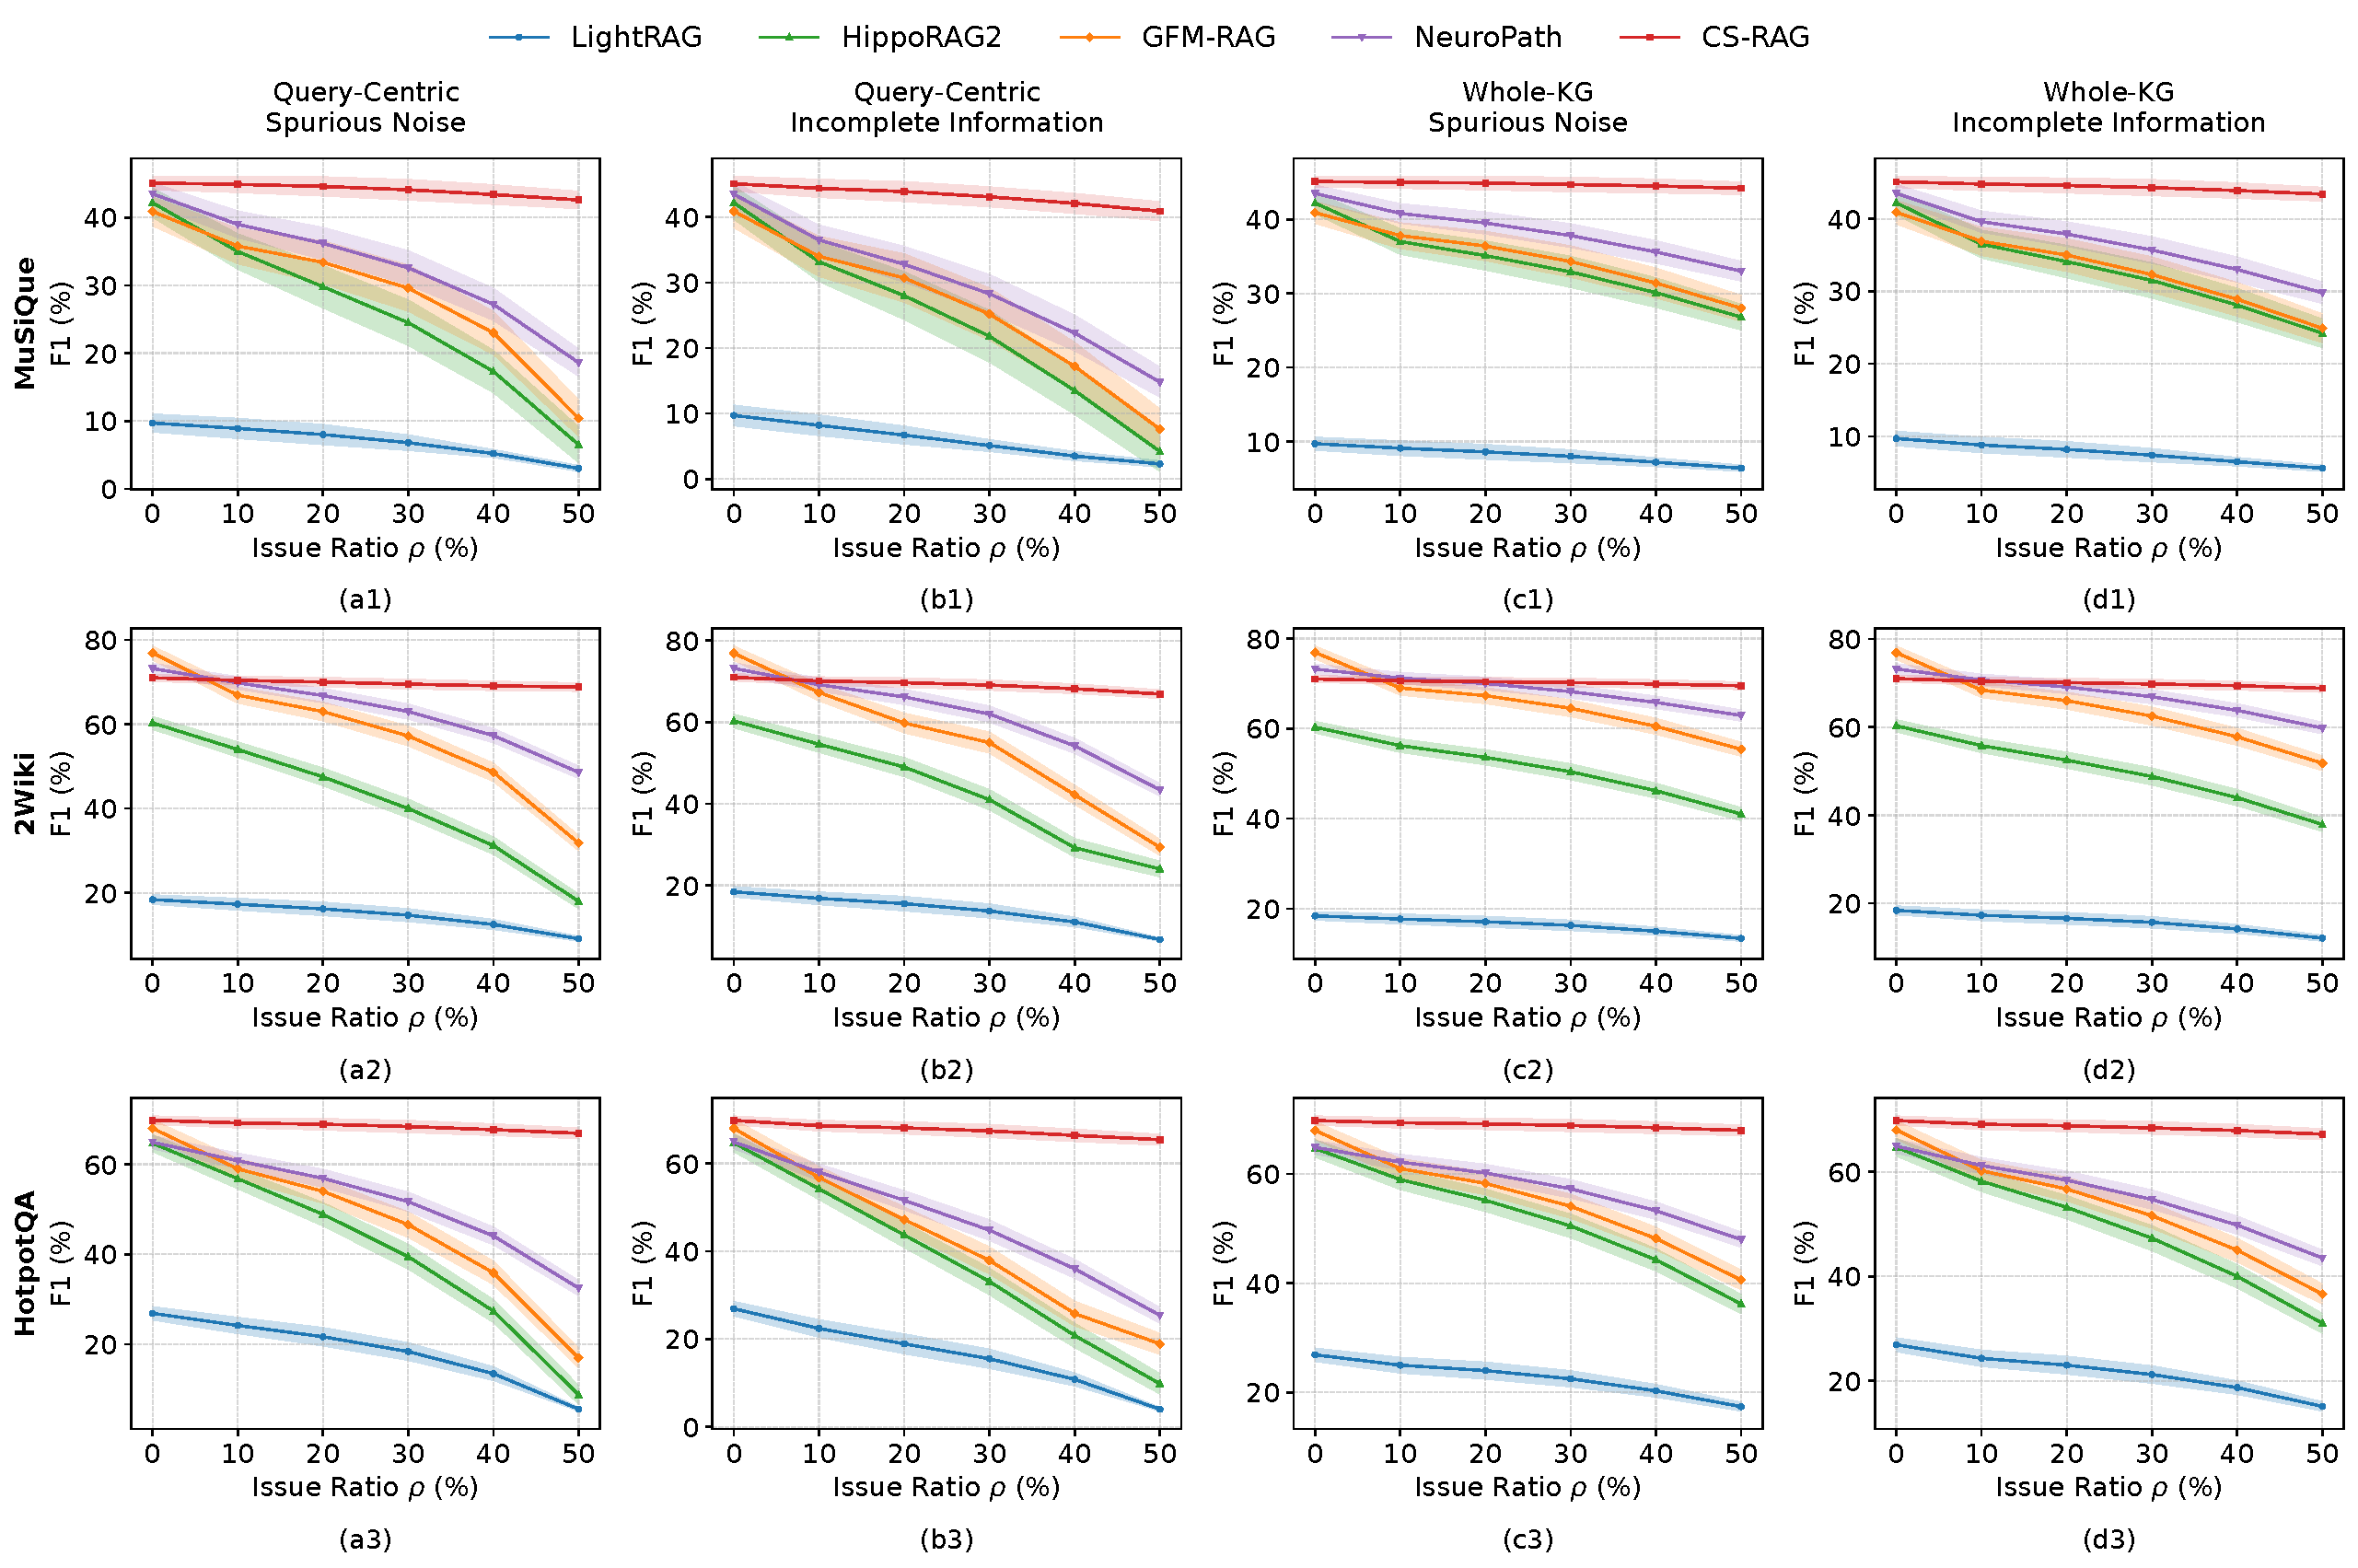
\includegraphics[width=0.99\linewidth]{Figs/robustness_3x4_f1_std.pdf} 
    \caption{F1 trends under controlled KG issue injection. Columns (a)--(d) correspond to Query-Centric Spurious Noise, Query-Centric Incomplete Information, Whole-KG Spurious Noise, and Whole-KG Incomplete Information, respectively. Rows 1--3 correspond to MuSiQue, 2Wiki, and HotpotQA, respectively. All baselines are evaluated by us by following their
released code. Lines show the mean F1, and shaded bands indicate the standard deviation over five runs.}
    \label{fig:robustness}
\end{figure*}


In this section, we evaluate robustness under controlled KG quality degradation to examine whether CS-RAG mitigates the two KG-induced challenges.  We consider two injection scopes: Query-Centric Issue Injection perturbs the local 2-hop neighborhoods around the entities, where injected issues directly affect the reasoning path, while Whole-KG Issue Injection perturbs the full query-specific KG, where issues are distributed more broadly across the graph. Within each scope, two issue modes are injected, namely spurious noise and incomplete information, with details provided in Appendix~\ref{app:issue_injection}. We use the GPT-4o-mini constructed KG as the base graph for controlled injection because it provides a relatively strong and stable starting point, allowing us to isolate the effect of each injected issue mode from naturally mixed builder errors. The issue ratio $\rho$ is varied over $\{0.1, 0.2, 0.3, 0.4, 0.5\}$. For each issue ratio, we repeat the injection process five times with different random seeds and report the mean F1 with one-standard-deviation bands in Figure~\ref{fig:robustness}.

\paragraph{Query-Centric Issue Injection} Figure~\ref{fig:robustness} (a)--(b) reports the results under query-centric injection. Across all three datasets, CS-RAG maintains nearly stable F1 as $\rho$ increases, while the baselines show clear performance degradation. Under spurious noise, baselines are more easily affected because corrupted but plausible triples can still participate in graph matching and propagation. NeuroPath is relatively more stable due to path-level selection, but its performance still drops as noisy local candidates enter the reasoning path. Under incomplete information, all baselines suffer from missing local bridges, since they tend to continue structural retrieval even when the required evidence chain is under-supported. CS-RAG remains much less affected because sufficiency checking and textual recovery reduce forced structural continuation.


\paragraph{Whole-KG Issue Injection} Figure~\ref{fig:robustness} (c)--(d) reports the results under whole-KG injection. Compared with query-centric injection, the degradation of baselines is generally more gradual, since only part of the injected issues directly intersects the reasoning path. However, their F1 still decreases as $\rho$ increases, showing that globally distributed KG issues can indirectly affect retrieval through repeated graph matching and propagation. This effect is more visible for graph-based baselines, which rely more heavily on the overall reliability of KG connectivity. CS-RAG remains nearly stable across issue ratios, indicating that constraint-based retrieval and sufficiency checking are still effective when KG issues are distributed broadly over the graph. These results show that the robustness of CS-RAG is not limited to local issue concentration, but also extends to whole-KG quality degradation.

% \begin{table*}[h]
% \centering
% \caption{F1 scores under Whole-KG Issue Injection on MuSiQue, 2WikiMultihopQA, and HotpotQA.}
% \label{tab:whole_kg}
% \scriptsize
% \setlength{\tabcolsep}{2.8pt}
% \resizebox{\textwidth}{!}{
% \begin{tabular}{l *{10}{c}|*{10}{c}|*{10}{c}}
% \toprule
% \multirow{3}{*}{\textbf{Method}} 
% & \multicolumn{10}{c|}{\textbf{MuSiQue}} 
% & \multicolumn{10}{c|}{\textbf{2WikiMultihopQA}} 
% & \multicolumn{10}{c}{\textbf{HotpotQA}} \\
% \cmidrule(lr){2-11} \cmidrule(lr){12-21} \cmidrule(lr){22-31}
% & \multicolumn{5}{c}{\textbf{Spurious Noise}} 
% & \multicolumn{5}{c|}{\textbf{Incomplete Information}}
% & \multicolumn{5}{c}{\textbf{Spurious Noise}} 
% & \multicolumn{5}{c|}{\textbf{Incomplete Information}}
% & \multicolumn{5}{c}{\textbf{Spurious Noise}} 
% & \multicolumn{5}{c}{\textbf{Incomplete Information}} \\
% \cmidrule(lr){2-6} \cmidrule(lr){7-11}
% \cmidrule(lr){12-16} \cmidrule(lr){17-21}
% \cmidrule(lr){22-26} \cmidrule(lr){27-31}
% & $\rho$=0.1 & $\rho$=0.2 & $\rho$=0.3 & $\rho$=0.4 & $\rho$=0.5
% & $\rho$=0.1 & $\rho$=0.2 & $\rho$=0.3 & $\rho$=0.4 & $\rho$=0.5
% & $\rho$=0.1 & $\rho$=0.2 & $\rho$=0.3 & $\rho$=0.4 & $\rho$=0.5
% & $\rho$=0.1 & $\rho$=0.2 & $\rho$=0.3 & $\rho$=0.4 & $\rho$=0.5
% & $\rho$=0.1 & $\rho$=0.2 & $\rho$=0.3 & $\rho$=0.4 & $\rho$=0.5
% & $\rho$=0.1 & $\rho$=0.2 & $\rho$=0.3 & $\rho$=0.4 & $\rho$=0.5 \\
% \midrule
% LightRAG   & 8.8  & 7.6  & 6.3  & 5.1  & 4.0  & 8.2  & 6.9  & 5.7  & 4.5  & 3.5
%            & 16.7 & 15.5 & 14.0 & 12.6 & 11.1 & 16.0 & 14.6 & 13.1 & 11.6 & 10.2
%            & 15.9 & 14.2 & 12.3 & 10.4 & 8.5  & 14.8 & 13.0 & 11.1 & 9.0  & 7.0 \\
% HippoRAG2  & 19.4 & 17.8 & 15.6 & 13.1 & 10.8 & 17.9 & 16.1 & 13.8 & 11.4 & 9.1
%            & 38.2 & 35.9 & 33.0 & 29.6 & 25.7 & 36.6 & 34.1 & 31.1 & 27.6 & 23.8
%            & 27.4 & 24.6 & 21.5 & 18.0 & 14.6 & 25.6 & 22.8 & 19.7 & 16.4 & 13.0 \\
% GFM-RAG    & 22.1 & 20.2 & 17.8 & 15.0 & 12.5 & 20.6 & 18.5 & 16.0 & 13.3 & 10.9
%            & 43.1 & 40.6 & 37.6 & 34.1 & 30.3 & 41.2 & 38.6 & 35.5 & 31.9 & 28.0
%            & 31.5 & 28.5 & 25.2 & 21.5 & 17.8 & 29.6 & 26.5 & 23.0 & 19.3 & 15.6 \\
% NeuroPath  & 31.8 & 29.9 & 27.5 & 24.8 & 21.9 & 30.4 & 28.4 & 25.9 & 23.1 & 20.2
%            & 62.0 & 60.1 & 57.8 & 55.1 & 52.1 & 60.8 & 58.7 & 56.1 & 53.1 & 49.9
%            & 49.8 & 47.6 & 44.8 & 41.4 & 37.6 & 47.9 & 45.2 & 42.0 & 38.2 & 34.0 \\
% \midrule
% CS-RAG      & \textbf{45.9} & \textbf{45.7} & \textbf{45.4} & \textbf{45.1} & \textbf{44.8}
%            & \textbf{45.7} & \textbf{45.4} & \textbf{45.1} & \textbf{44.7} & \textbf{44.4}
%            & \textbf{73.7} & \textbf{73.4} & \textbf{73.1} & \textbf{72.7} & \textbf{72.3}
%            & \textbf{73.5} & \textbf{73.2} & \textbf{72.8} & \textbf{72.4} & \textbf{72.0}
%            & \textbf{69.5} & \textbf{69.2} & \textbf{68.8} & \textbf{68.4} & \textbf{67.9}
%            & \textbf{69.2} & \textbf{68.8} & \textbf{68.4} & \textbf{67.9} & \textbf{67.4} \\
% \bottomrule
% \end{tabular}
% }
% \end{table*}


\subsection{Ablation Study}
\label{sec:ablation}

\begin{wraptable}{r}{0.5\linewidth}
\vspace{-0.0em}
    \centering
    \scriptsize
    \setlength{\tabcolsep}{2pt}
    \caption{Ablation results of EM (\%) and F1 (\%) under different builders on HotpotQA.}
    \label{tab:ablation_main}
    \begin{tabular}{lcccccc}
        \toprule
        \multirow{2}{*}{Method} &
        \multicolumn{2}{c}{\textbf{GPT-4o-mini}} &
        \multicolumn{2}{c}{\textbf{Llama-3.1-70B}} &
        \multicolumn{2}{c}{\textbf{Qwen-3-14B}} \\
        \cmidrule(lr){2-3} \cmidrule(lr){4-5} \cmidrule(lr){6-7}
        & EM & F1 & EM & F1 & EM & F1 \\
        \midrule
        CS-RAG & 54.3 & 69.8 & 53.4 & 68.9 & 52.7 & 68.0 \\
        \midrule
        \multicolumn{7}{l}{\textit{Constraint-based Retrieval}} \\
        w/o Planner & 49.8 & 64.0 & 47.1 & 61.3 & 45.6 & 59.3 \\
        w/o Relation & 51.5 & 66.4 & 50.4 & 64.8 & 49.3 & 63.8 \\
        w/o Constraint & 51.0 & 65.8 & 50.0 & 64.3 & 48.6 & 62.7 \\
        \midrule
        \multicolumn{7}{l}{\textit{Sufficiency-Guided Propagation and Recovery}} \\
        w/o Check & 50.3 & 64.7 & 47.8 & 62.0 & 46.5 & 60.2 \\
        w/o Dist & 52.1 & 66.7 & 50.5 & 65.2 & 49.5 & 63.5 \\
        \bottomrule
    \end{tabular}
    \vspace{-0.0em}
\end{wraptable}

We conduct ablations on HotpotQA to evaluate two core parts of CS-RAG: constraint-based retrieval and sufficiency checking. For constraint-based retrieval, w/o Planner removes atomic constraint planning and uses the original query as a single semantic retrieval request, which evaluates whether planning itself is necessary. 
w/o Constraint keeps the LLM-generated atomic constraints but replaces fine-grained constraint retrieval with coarse semantic matching, which evaluates the necessity of constraint-aware execution after planning. w/o Relation removes relation alignment and reranks candidates using only entity information to assess the contribution of relation-level matching. 
For Sufficiency-Guided Propagation and Recovery, w/o Check disables the sufficiency check and always propagates structural candidates to subsequent hops, examining the value of sufficiency verification. 
w/o Dist replaces the distribution-based criterion with a fixed binary score threshold, classifying a constraint as resolved when the highest score exceeds 0.5 and unresolved otherwise. Each variant modifies one targeted design choice or module while keeping the remaining pipeline unchanged.



% \begin{wraptable}{r}{0.53\linewidth}
% \vspace{-0.5em}
%     \centering
%     \scriptsize
%     \setlength{\tabcolsep}{4pt}
%     \caption{Ablation results of EM (\%) and F1 (\%) under different builders on MuSiQue.}
%     \label{tab:ablation_main}
%     \begin{tabular}{lcccccc}
%         \toprule
%         \multirow{2}{*}{Method} &
%         \multicolumn{2}{c}{\textbf{GPT-4o-mini}} &
%         \multicolumn{2}{c}{\textbf{Llama-3.1-70B}} &
%         \multicolumn{2}{c}{\textbf{Qwen-3-14B}} \\
%         \cmidrule(lr){2-3} \cmidrule(lr){4-5} \cmidrule(lr){6-7}
%         & EM & F1 & EM & F1 & EM & F1 \\
%         \midrule
%         CS-RAG & 56.9 & 69.9 & 53.8 & 66.5 & 52.3 & 65.0 \\
%         \midrule
%         \multicolumn{7}{l}{\textit{Constraint-based Retrieval}} \\
%         w/o Constraint & 52.4 & 64.1 & 47.5 & 58.9 & 45.2 & 56.3 \\
%         w/o Relation & 54.1 & 66.5 & 50.8 & 62.4 & 48.9 & 60.8 \\
%         w/o Placeholder & 53.6 & 65.9 & 50.4 & 61.9 & 48.2 & 59.7 \\
%         \midrule
%         \multicolumn{7}{l}{\textit{Sufficiency Check}} \\
%         w/o Check & 52.9 & 64.8 & 48.2 & 59.6 & 46.1 & 57.2 \\
%         w/o Dist & 54.7 & 66.8 & 50.9 & 62.8 & 49.1 & 60.5 \\
%         \bottomrule
%     \end{tabular}
%     \vspace{-0.5em}
% \end{wraptable}

Table~\ref{tab:ablation_main} shows that the ablated variants fail in different ways. 
w/o Planner suffers the largest drop because treating the original question as a single semantic retrieval request removes explicit hop-wise targets and intermediate dependencies. 
w/o Constraint further shows that planning alone is insufficient, since coarse semantic matching cannot enforce fine-grained constraint execution and is more likely to admit target-misaligned evidence. 
w/o Relation causes a consistent drop across builders, indicating that relation matching helps distinguish entity-related candidates from constraint-compatible evidence. 
w/o Check forces propagation from ambiguous candidate pools, making the pipeline more vulnerable to retrieval hallucination under weaker builders. 
w/o Dist also degrades performance, suggesting that binary decisions ignore distributional ambiguity among competing candidates and are less reliable than distribution-based sufficiency scoring. Additional ablation results for other modules are provided in Appendix~\ref{appsec:ablation}.

\subsection{Hyperparameter Study}
\label{appsec:rq7_hparam}

% \begin{figure*}[h]
%     \centering
%     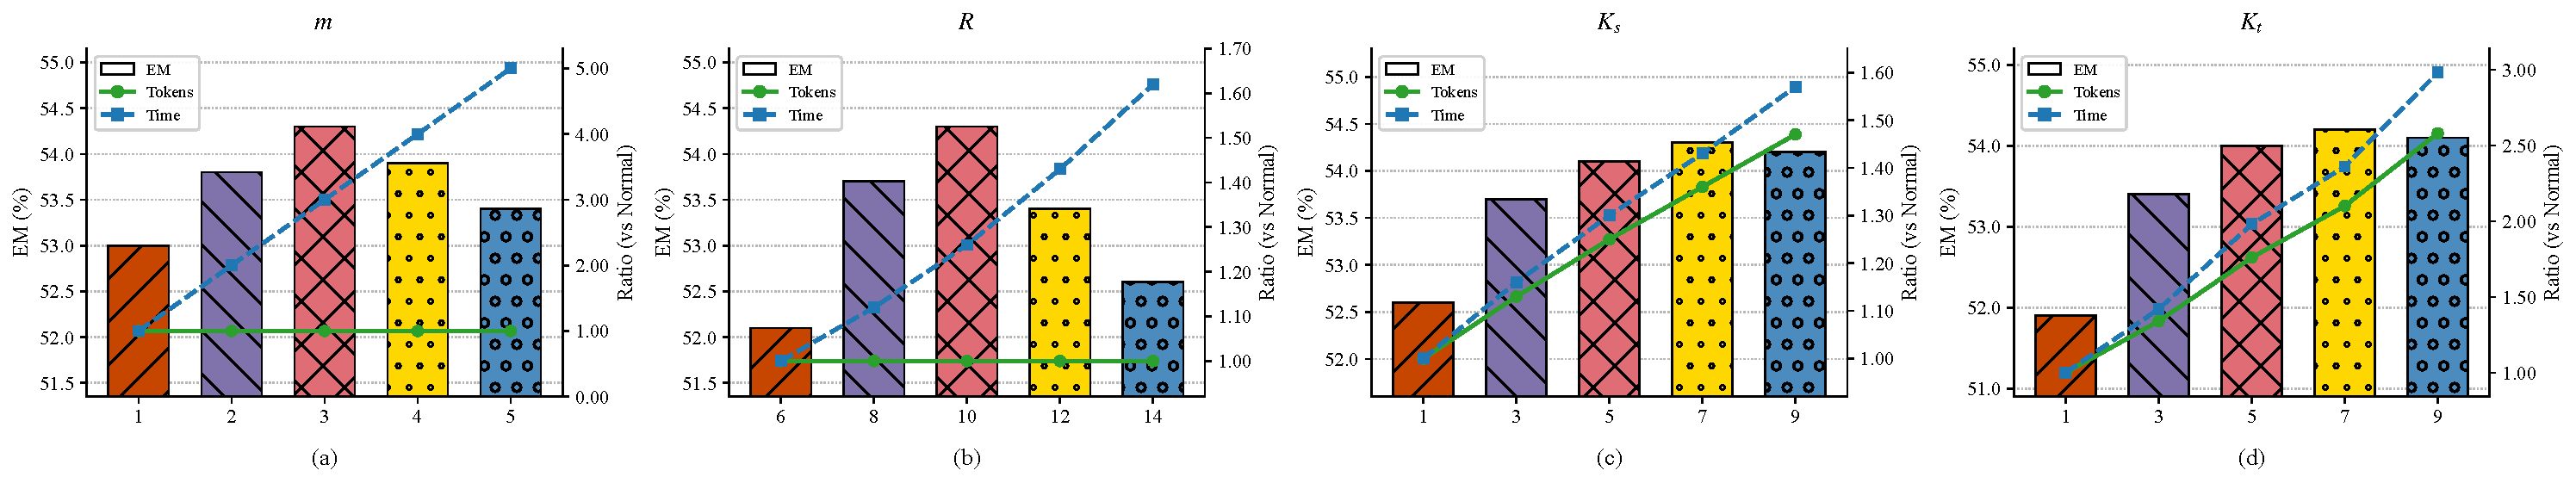
\includegraphics[width=1.0\linewidth]{Figs/hyperparam_2x2_final.pdf}
%     \caption{Hyperparameter sensitivity of CS-RAG. We vary (a) the sufficiency check threshold $\gamma$, (b) the number of relation variants $m$, (c) the structural candidate budget $K_s$, and (d) the textual recovery budget $K_t$, reporting EM and the QA token ratio.}
%     \label{fig:hparam}
% \end{figure*}

% \begin{wrapfigure}{r}{0.58\columnwidth}
%     \vspace{-0.8em}
%     \centering
%     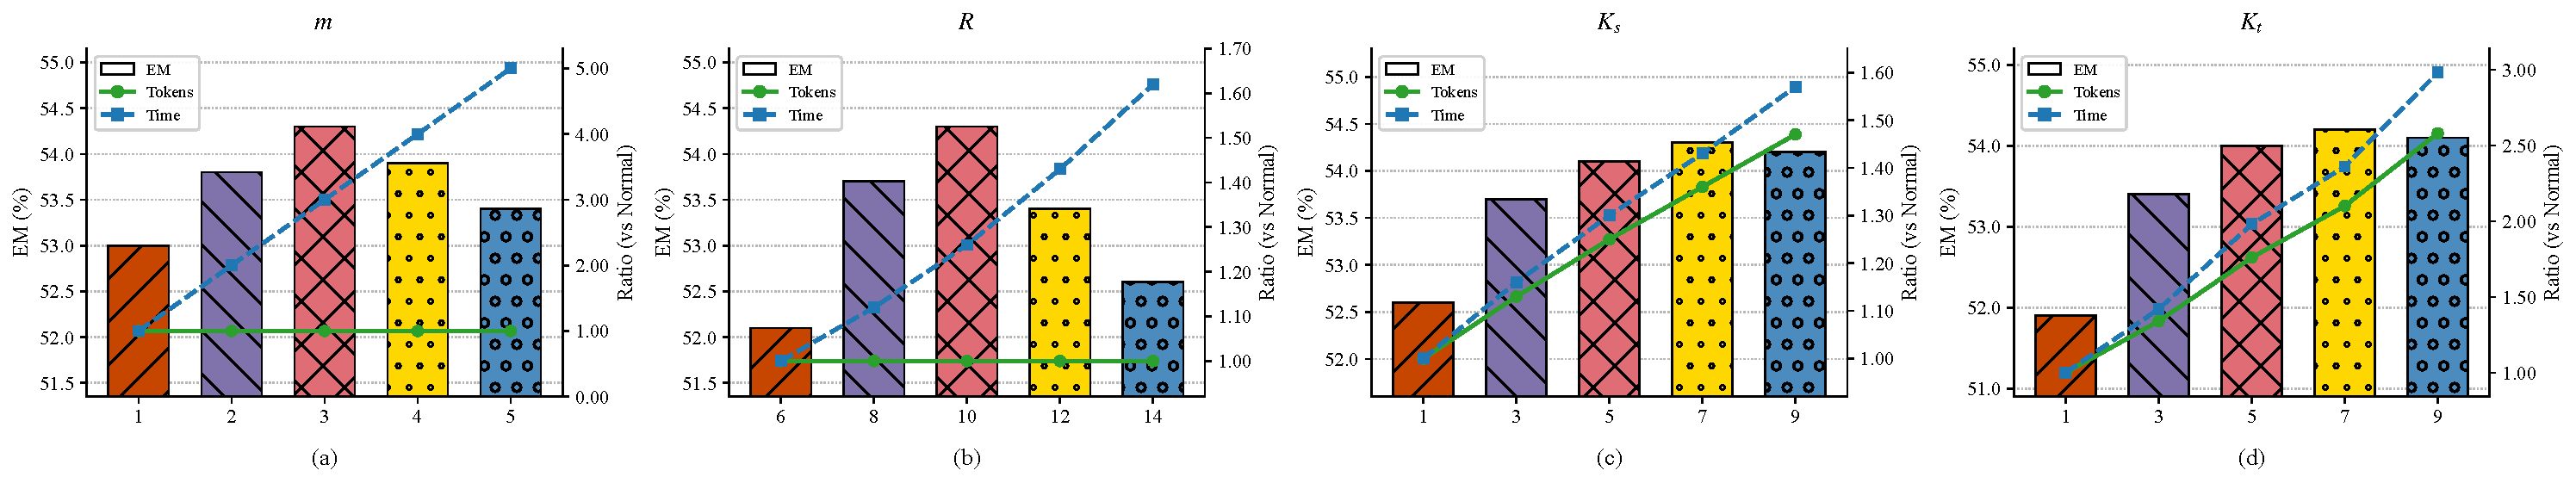
\includegraphics[width=\linewidth]{Figs/hyperparam_2x2_final.pdf}
%     \caption{Hyperparameter sensitivity of CS-RAG. We vary (a) $\gamma$, (b) relation variants $m$, (c) structural candidate budget $K_s$, and (d) textual recovery budget $K_t$, reporting EM and QA token ratio.}
%     \label{fig:hparam}
%     \vspace{-0.8em}
% \end{wrapfigure}

We analyze hyperparameter sensitivity of CS-RAG in this section. 
For constraint-based retrieval, we vary the number of relation variants $m$, the relation-aligned candidate budget $R$, and the structural candidate budget $K_s$. 
For sufficiency-guided propagation and recovery, we vary the textual recovery budget $K_t$ and the sufficiency threshold $\gamma$. Table~\ref{tab:gamma_sensitivity} shows that $\gamma$ controls a dataset-dependent balance between structural propagation and textual recovery. 
\begin{wraptable}{r}{0.48\textwidth}
\vspace{-0.0em}
\centering
\scriptsize
\setlength{\tabcolsep}{2pt}
\caption{Effect of the representative $\gamma$-values from the searched range across datasets. Res. denotes the ratio of executed constraint hops classified as resolved. Time measures online retrieval latency, and Tokens denotes the retrieved evidence tokens fed into the final QA. \textbf{Bold} indicates the trade-off setting used for reporting the results in the main experiments.}
\label{tab:gamma_sensitivity}
\resizebox{\linewidth}{!}{
\begin{tabular}{llccccc}
\toprule
Dataset & $\gamma$ & Res. (\%) & EM (\%)  & F1 (\%)  & Time(s) & Tokens \\
\midrule
\multirow{5}{*}{MuSiQue}
& 1.2 & 25.6 & 34.1 & 47.9 & 8.8 & 5.4k\\
& \textbf{1.5} & \textbf{44.9} & \textbf{32.2} & \textbf{45.1} & \textbf{6.3} & \textbf{3.9k} \\
& 1.8 & 57.7 & 30.2 & 42.1 & 5.8 & 3.2k \\
& 2.1 & 69.8 & 27.4 & 39.8 & 4.2 & 2.6k \\
& 2.4 & 80.9 & 25.7 & 35.2 & 3.3 & 1.9k \\
\midrule
\multirow{5}{*}{2Wiki}
& 1.2 & 24.2 & 61.9 & 66.2 & 3.0 & 1.9k \\
& 1.4 & 41.0 & 62.8 & 69.1 & 2.3 & 1.4k \\
& \textbf{1.6} & \textbf{45.8} & \textbf{63.0} & \textbf{71.0} & \textbf{1.7} & \textbf{1.1k} \\
& 1.8 & 79.1 & 63.6 & 70.4 & 1.4 & 0.9k \\
& 2.0 & 86.7 & 60.8 & 68.5 & 1.3 & 0.8k \\
\midrule
\multirow{5}{*}{HotpotQA}
& 1.2 & 20.4 & 57.7 & 72.1 & 3.2 & 2.0k \\
& 1.6 & 44.1 & 55.6 & 70.1 & 2.6 & 1.5k \\
& \textbf{2.0} & \textbf{61.5} & \textbf{54.3} & \textbf{69.8} & \textbf{2.2} & \textbf{1.2k} \\
& 2.4 & 74.6 & 51.9 & 66.7 & 1.9 & 1.0k \\
& 2.8 & 83.4 & 47.6 & 62.4 & 1.7 & 0.8k \\
\bottomrule
\end{tabular}
}
\vspace{-0.8em}
\end{wraptable}
As $\gamma$ increases, the resolved-hop rate rises and both online retrieval time and inference tokens decrease, because more constraints are allowed to continue through structural propagation rather than being routed to textual recovery. However, the QA trend differs across datasets. 
On MuSiQue, smaller $\gamma$ yields stronger EM and F1, but it also introduces substantially higher latency and more final-context tokens. This pattern suggests that MuSiQue benefits from routing uncertain hops to textual recovery and retaining additional evidence, while its longer constraint chains and richer variable dependencies make the induced overhead more pronounced. HotpotQA follows a similar but milder accuracy-efficiency trade-off, where smaller \(\gamma\) improves QA performance at a higher online cost, but the gain is less pronounced than on MuSiQue. For 2Wiki, performance improves up to a moderate threshold and then decreases when $\gamma$ becomes larger. 
This is consistent with its shorter reasoning structure and larger proportion of directly executable hops, where overly permissive structural propagation may accept weak or ambiguous bindings rather than providing useful additional evidence. 
These results indicate that $\gamma$ should be selected according to the dataset-specific trade-off among structural propagation, textual recovery, and online cost. 
The other results for $m$, $R$, $K_s$, and $K_t$ are provided in Appendix~\ref{appsec: Hyperparameter_detail}.



\subsection{Failure Analysis.}

We further analyze two representative failure cases in Appendix~\ref{app:failure_analysis}, corresponding to planner errors and insufficient evidence. 
In the first case, the planner omits an intermediate bridge variable, causing the generated constraints to retrieve evidence around the wrong entity. 
This shows that planner quality remains important for CS-RAG, since an incorrect plan can specify the wrong retrieval target and affect subsequent evidence acquisition. 
Nevertheless, the statistics in Appendix~\ref{app:planner_error_stats} show low error rates at both the hop and plan levels, indicating that GPT-4o-mini has enough ability to provide sufficiently reliable plans for most queries. 
In the second case, CS-RAG fails when the required bridge evidence is absent or too implicit in both the KG and the recovered text pool. 
This indicates that when both the KG and recovered passages mention only related entities without the required relation, further improvement depends on recovering the missing bridge evidence itself.

% \subsection{More Analyses}
% Additional analyses, including supplementary ablations, hyperparameter sensitivity, constraint statistics, sufficiency-check correctness, planner-error statistics, failure analysis, and case studies, are reported in Appendix~\ref{Supplementary Results}.

\section{Conclusion}

In this paper, we first analyze KG construction outcomes across different LLM-based builders and identify two recurring issue modes, spurious noise and incomplete information. Then we propose CS-RAG, a robust GraphRAG framework for multi-hop retrieval on imperfect LLM-constructed KGs. CS-RAG mitigates two issue-induced retrieval failures: retrieval drift caused by spurious noise, and retrieval hallucination caused by incomplete information. Specifically, constraint-based retrieval grounds each hop in fine-grained anchor and relation constraints to reduce drift toward structurally plausible but unsupported evidence, while sufficiency-guided propagation and textual recovery reduce the chance that incomplete KGs force hallucinated structural continuations. Experiments on three multi-hop QA benchmarks show that CS-RAG achieves stronger robustness across different KG builders and under controlled KG issue injection.


\bibliography{mybib}
\bibliographystyle{plainnat}

%%%%%%%%%%%%%%%%%%%%%%%%%%%%%%%%%%%%%%%%%%%%%%%%%%%%%%%%%%%%%%%%%%%%%%%%%%%%%%%
%%%%%%%%%%%%%%%%%%%%%%%%%%%%%%%%%%%%%%%%%%%%%%%%%%%%%%%%%%%%%%%%%%%%%%%%%%%%%%%
% APPENDIX
%%%%%%%%%%%%%%%%%%%%%%%%%%%%%%%%%%%%%%%%%%%%%%%%%%%%%%%%%%%%%%%%%%%%%%%%%%%%%%%
%%%%%%%%%%%%%%%%%%%%%%%%%%%%%%%%%%%%%%%%%%%%%%%%%%%%%%%%%%%%%%%%%%%%%%%%%%%%%%%
\newpage
\appendix %一定要放在\bibliography{...}之后
\onecolumn

\section{Representative Incorrect Patterns}
\label{app:issue_patterns}

In this section, we provide a detailed description of six representative incorrect patterns observed in builder-extracted tuples.

\paragraph{Over-generalized Relation.}
This pattern refers to cases where the extracted tuple replaces a specific relation stated in the source evidence with a broader or less informative relation.
For example, the sentence states that \emph{Jeremy Renner was nominated for the Academy Award for Best Actor for his role in The Hurt Locker}, while the extracted tuple is effectively \emph{Jeremy Renner -- associated with -- Academy Award for Best Actor}. The extracted relation preserves a topical connection between the two entities, but it drops the precise nomination relation required by the evidence.

\paragraph{Mis-bound Relation.}
This pattern refers to cases where the extracted tuple links entities that appear in the same sentence, but the relation between them is not actually expressed in the source evidence.
For example, the sentence states that \emph{Karl Marx was born in Trier and studied at the University of Bonn}, while the extracted tuple becomes \emph{Trier -- related\_to -- Bonn}. Although both entities are mentioned, the sentence does not express such a direct relation.

\paragraph{Semantic Flip.}
This pattern refers to cases where the extracted tuple reverses or distorts the original semantic meaning of the source evidence.
For example, the sentence says that \emph{the report doesn't find that Drug A is associated with increased risk of stroke}, while the extracted tuple becomes \emph{Drug A -- associated with -- increased\_risk\_stroke}. The tuple remains topically related, but its meaning is opposite to that of the source sentence.

\paragraph{Missing Bridge Edge.}
This pattern refers to cases where the extracted tuples fail to provide a necessary connection between two pieces of evidence, leaving the reasoning chain structurally incomplete.
For example, the graph contains \emph{iPhone 13 -- powered\_by -- A15 Bionic} and \emph{Apple Inc. -- headquartered\_in -- Cupertino}, but misses the bridge \emph{A15 Bionic -- designed\_by -- Apple Inc.}. As a result, the intended multi-hop connection cannot be completed.

\paragraph{Dropped Qualifier.}
This pattern refers to cases where the extracted tuple preserves the main fact but omits a qualifier that is necessary for a complete or precise interpretation.
For example, the sentence states that \emph{In 2002, Elon Musk founded SpaceX}, while the extracted tuple keeps \emph{Elon Musk -- founded -- SpaceX} but drops the qualifier \emph{in 2002}. The extracted fact is only partially preserved.

\paragraph{Others.}
This pattern refers to a case set of low-frequency incorrect cases that usually have limited influence on downstream retrieval.
For example, one case is incomplete entity surface extraction, where the extracted entity name is only partially preserved, such as extracting \emph{Musk} instead of \emph{Elon Musk}. Another case is off-chain redundant tuple extraction, where the builder extracts an additional tuple that is loosely related to the source sentence but falls outside the evidence chain required by the query.  For example, from a sentence used to support \emph{No Cross, No Crown -- written during imprisonment in -- Tower of London}, the builder may additionally extract \emph{Tower of London -- located\_in -- London}. This tuple is sentence-related, but it does not contribute to the target reasoning chain.
 
\section{Justification of $N_{\mathrm{eff}}$}
\label{app:neff}

This appendix provides theoretical support for the sufficiency check.
Here $\{p_{i,c}\}_{c\in\mathcal{C}_i^{top}}$ is the normalized candidate distribution computed from cross-encoder scores, and $\mathcal{C}_i^{top}$ is the refined structural candidate pool for constraint $\tau_i$.

\subsection{Properties of $N_{\mathrm{eff}}$}

Let $p$ be any probability distribution on a finite candidate set $\mathcal{C}$ with $n=|\mathcal{C}|$, and define
\begin{equation}
N_{\mathrm{eff}}(p) \triangleq \frac{1}{\sum_{c\in\mathcal{C}} p_c^2}.
\label{eq:app_neff_general}
\end{equation}
Since $\sum_{c} p_c^2=\|p\|_2^2$ increases when probability concentrates on fewer candidates, $N_{\mathrm{eff}}(p)$ acts as an effective number of competing candidates.

\begin{lemma}[Range and extremal cases]
\label{lem:range}
For any distribution $p$ on $\mathcal{C}$,
\begin{equation}
1 \le N_{\mathrm{eff}}(p) \le n.
\label{eq:app_range}
\end{equation}
Moreover, $N_{\mathrm{eff}}(p)=1$ if $p$ is a point mass, and $N_{\mathrm{eff}}(p)=n$ if $p$ is uniform.
\end{lemma}
\begin{proof}
Since $\sum_c p_c^2 \le \sum_c p_c = 1$, we have $N_{\mathrm{eff}}(p)\ge 1$.
For the upper bound, Cauchy--Schwarz gives
\[
\Big(\sum_{c\in\mathcal{C}} p_c\Big)^2 \le n \sum_{c\in\mathcal{C}} p_c^2
\ \Rightarrow\
1 \le n \sum_c p_c^2
\ \Rightarrow\
N_{\mathrm{eff}}(p) \le n.
\]
The extremal cases follow by direct substitution.
\end{proof}

\subsection{Threshold interpretation for sufficiency check}

We next show that the sufficiency check $N_{\mathrm{eff}}(p)\le\gamma$ implies the existence of a dominant candidate.


\begin{lemma}[Lower bound on the top probability]
\label{lem:pmax}
Let $p_{\max}=\max_{c\in\mathcal{C}} p_c$. For any distribution $p$ on $\mathcal{C}$,
\begin{equation}
p_{\max} \ge \sum_{c\in\mathcal{C}} p_c^2 = \frac{1}{N_{\mathrm{eff}}(p)}.
\label{eq:app_pmax_lb}
\end{equation}
\end{lemma}
\begin{proof}
For every $c$, $p_c \le p_{\max}$ implies $p_c^2 \le p_{\max}p_c$.
Summing over $c$ yields
\[
\sum_{c\in\mathcal{C}} p_c^2 \le p_{\max}\sum_{c\in\mathcal{C}} p_c = p_{\max}.
\]
\end{proof}

\begin{proposition}[Sufficiency check guarantees a dominant candidate]
\label{prop:sufficiency}
Consider a constraint $\tau_i$ with candidate pool $\mathcal{C}_i^{top}$ and distribution $\{p_{i,c}\}$.
If the sufficiency check accepts $\tau_i$, i.e., $N_{\mathrm{eff}}(\tau_i)\le \gamma$, then
\begin{equation}
\max_{c\in\mathcal{C}_i^{top}} p_{i,c} \ge \frac{1}{\gamma}.
\label{eq:app_accept_lb}
\end{equation}
\end{proposition}
\begin{proof}
By Lemma~\ref{lem:pmax}, $\max_c p_{i,c} \ge 1/N_{\mathrm{eff}}(\tau_i)$.
If $N_{\mathrm{eff}}(\tau_i)\le\gamma$, then $1/N_{\mathrm{eff}}(\tau_i)\ge 1/\gamma$, yielding Eq.~\ref{eq:app_accept_lb}.
\end{proof}

Proposition~\ref{prop:sufficiency} explains why $N_{\mathrm{eff}}$ is a suitable score for sufficiency check in CS-RAG.
When $N_{\mathrm{eff}}$ is large, the candidate distribution lacks a dominant option and any structural binding is inherently ambiguous.
Applying the threshold $N_{\mathrm{eff}}(\tau_i)\le\gamma$ therefore suppresses hallucinated bindings by allowing structural propagation only when the distribution admits a clear winner.

% \section{Algorithm}
% \label{app:algorithm}

% Algorithm~\ref{alg:CS-RAG_basic} summarizes the inference pipeline of CS-RAG.

% \begin{algorithm}[t]
% \caption{CS-RAG Inference (Basic Steps)}
% \label{alg:CS-RAG_basic}
% \begin{algorithmic}[1]
% \Require query $q$, KG $\mathcal{G}$, passages $U(q)$
% \Require planner $\mathrm{Plan}(\cdot)$, cross-encoder $\mathrm{CE}(\cdot)$, embedder $\mathrm{Enc}(\cdot)$
% \Require structural hyperparameters $E, R, K_s$, textual hyperparameters $K_t', K_t$, threshold $\gamma$
% \Ensure answer $\hat{y}$

% \State obtain constraint plan $\mathcal{P}=\langle \tau_1,\ldots,\tau_k\rangle$ and relation variants $\{\mathcal{R}_i\}_{i=1}^k$ from $\mathrm{Plan}(q)$
% \State initialize resolved set $\mathcal{P}_R\leftarrow\emptyset$, unresolved set $\mathcal{P}_U\leftarrow\emptyset$
% \State initialize binding map $\mathcal{E}_b(\cdot)\leftarrow\emptyset$ and evidence map $\mathcal{T}^{txt}(\tau_i)\leftarrow\emptyset$ for all $i$

% \State initialize queue $\mathcal{Q}\leftarrow \{\,\tau_i\in\mathcal{P}\mid |\{h_i,t_i\}\cap\mathcal{V}|=1\,\}$ \Comment{single-variable constraints}
% \State initialize set $\mathcal{P}_2\leftarrow \{\,\tau_i\in\mathcal{P}\mid h_i\in\mathcal{V},\, t_i\in\mathcal{V}\,\}$ \Comment{two-variable constraints}

% \While{$\mathcal{Q}\neq\emptyset$}
%     \State pop a constraint $\tau_i$ from $\mathcal{Q}$
%     \State $(\mathcal{C}_i^{top}, \{p_{i,c}\}) \leftarrow \Call{StructRetrieve}{q,\tau_i,\mathcal{R}_i,\mathcal{G},\mathcal{E}_b,E,R,K_s,\mathrm{CE}}$
%     \State compute $N_{\mathrm{eff}}(\tau_i)=\big(\sum_{c\in\mathcal{C}_i^{top}} p_{i,c}^2\big)^{-1}$
%     \If{$N_{\mathrm{eff}}(\tau_i)\le \gamma$}
%         \State add $\tau_i$ to $\mathcal{P}_R$
%         \State update $\mathcal{E}_b(\cdot)$ using $\mathcal{C}_i^{top}$ (Eq.~13--14)
%         \State collect provenance passages of triples in $\mathcal{C}_i^{top}$ as $\mathcal{T}^{txt}(\tau_i)$
%         \State \Call{ActivatePropagation}{$\mathcal{P}_2,\mathcal{E}_b,\mathcal{Q}$} \Comment{turn newly anchorable two-variable constraints into single-variable ones}
%     \Else
%         \State add $\tau_i$ to $\mathcal{P}_U$
%     \EndIf
% \EndWhile

% \ForAll{$\tau_u \in \mathcal{P}_U$} \Comment{textual recovery for unresolved constraints}
%     \State compute $S_{txt}(\tau_u,d)=\cos(\mathrm{Enc}(\mathrm{Lin}(\tau_u)),\,\mathrm{Enc}(d))$ for $d\in U(q)$
%     \State $\hat{U}_u \leftarrow \mathrm{top}\text{-}K_t'\big(S_{txt}(\tau_u,d)\big)$
%     \State rerank $d\in\hat{U}_u$ by $s_{u,d}=\mathrm{CE}\big(q \,\Vert\, \mathrm{Lin}(\tau_u)\,\Vert\, d\big)$
%     \State set $\mathcal{T}^{txt}(\tau_u)\leftarrow \mathrm{top}\text{-}K_t$ passages under $s_{u,d}$
% \EndFor

% \State pack evidence blocks $B_q=\{\, [\,\mathrm{Lin}(\tau_i),\,\mathcal{T}^{txt}(\tau_i)\,] \,\}_{i=1}^{k}$
% \State generate answer $\hat{y}$ conditioned on $q$ and $B_q$
% \State \Return $\hat{y}$
% \end{algorithmic}
% \end{algorithm}

% \begin{algorithm}[t]
% \caption{StructRetrieve and Propagation Helpers}
% \label{alg:CS-RAG_helpers}
% \begin{algorithmic}[1]
% \Function{StructRetrieve}{$q,\tau_i,\mathcal{R}_i,\mathcal{G},\mathcal{E}_b,E,R,K_s,\mathrm{CE}$}
%     \State obtain anchor set $\mathcal{E}^{anchor}_i$ from the grounded endpoint of $\tau_i$ using top-$E$ matching (Eq.~3)
%     \State if the grounded endpoint is a variable with $\mathcal{E}_b(v)\neq\emptyset$, set $\mathcal{E}^{anchor}_i\leftarrow \mathcal{E}_b(v)$
%     \State enumerate one-hop triples around $\mathcal{E}^{anchor}_i$ to form $\mathcal{C}_i$ (Eq.~4)
%     \State keep top-$R$ triples under relation alignment $S_{rel}(\cdot,\mathcal{R}_i)$ to obtain $\mathcal{C}_i^{init}$ (Eq.~5)
%     \State rerank $c\in\mathcal{C}_i^{init}$ by $z_{i,c}=\mathrm{CE}\big(q \,\Vert\, \mathrm{Lin}(\tau_i)\,\Vert\, \mathrm{Lin}(c)\big)$ (Eq.~6)
%     \State keep top-$K_s$ triples as $\mathcal{C}_i^{top}$ and normalize $\{z_{i,c}\}$ into $\{p_{i,c}\}$ (Eq.~7)
%     \State \Return $(\mathcal{C}_i^{top}, \{p_{i,c}\})$
% \EndFunction

% \Function{ActivatePropagation}{$\mathcal{P}_2,\mathcal{E}_b,\mathcal{Q}$}
%     \ForAll{$\tau_j=(v_a,r_j,v_b)\in\mathcal{P}_2$}
%         \If{$\mathcal{E}_b(v_a)\neq\emptyset$ \textbf{or} $\mathcal{E}_b(v_b)\neq\emptyset$}
%             \State push $\tau_j$ into $\mathcal{Q}$ and remove it from $\mathcal{P}_2$
%         \EndIf
%     \EndFor
% \EndFunction
% \end{algorithmic}
% \end{algorithm}


% \begin{algorithm}[t]
% \caption{CS-RAG Inference (Condensed)}
% \label{alg:CS-RAG_condensed}
% \begin{algorithmic}[1]
% \Require Query $q$; KG $G=(\mathcal{E},\mathcal{T})$ with provenance; passages $U(q)$;
% planner $\mathcal{P}$; reranker $\mathrm{CE}(\cdot)$; budgets $(E_{\max},R_1,K)$; gate $(\gamma,\epsilon)$
% \Ensure Answer $\hat{y}$ and constraint-aligned context $B_q$

% \State $(\langle \tau_1,\dots,\tau_k\rangle,\{R_i\},E_q,V)\gets \mathcal{P}(q)$
% \State $P_1\gets$ single-variable constraints;\ \ $P_2\gets$ two-variable constraints;\ \ $E_b(\cdot)\gets\emptyset$
% \State $\mathcal{P}_R\gets\emptyset,\ \mathcal{P}_U\gets\emptyset$;\ \ $E^{txt}_i\gets\emptyset\ \forall i$

% \Function{\textsc{StructStep}}{$\tau$} \Comment{constraint-anchored structural retrieval + gating}
%     \State $E^{anchor}\gets \textsc{topE}(\mathcal{E},\textsc{AnchorSim}(\tau),E_{\max})$
%     \State $C\gets \textsc{OneHop}(\mathcal{T},E^{anchor})$
%     \State $C\gets \textsc{topR}(C,\textsc{RelSim}(\tau,R_\tau),R_1)$
%     \State $C\gets \textsc{topK}(C,\mathrm{CE}(q,\tau,c),K)$
%     \State $p_c\propto (s_c-\min s+\epsilon)$;\ \ $N_{\mathrm{eff}}(\tau)\gets 1/\sum_{c\in C}p_c^2$
%     \State \Return $(C,N_{\mathrm{eff}}(\tau))$
% \EndFunction

% \vspace{2pt}
% \ForAll{$\tau_i\in P_1$ \textbf{in order}}
%     \State $(C_i,n_i)\gets \textsc{StructStep}(\tau_i)$
%     \If{$n_i\le \gamma$}
%         \State $\mathcal{P}_R\gets \mathcal{P}_R\cup\{\tau_i\}$;\ \ $E_b(\cdot)\gets \textsc{UpdateBindings}(E_b,C_i)$
%         \State $E^{txt}_i\gets \textsc{ProvenanceText}(C_i,E_b)$
%     \Else
%         \State $\mathcal{P}_U\gets \mathcal{P}_U\cup\{\tau_i\}$
%     \EndIf
% \EndFor

% \vspace{2pt}
% \State $\texttt{changed}\gets \texttt{true}$
% \While{$\texttt{changed}$} \Comment{binding propagation on $P_2$}
%     \State $\texttt{changed}\gets \texttt{false}$
%     \ForAll{$\tau_j\in P_2$}
%         \If{\textsc{Bindable}$(\tau_j,E_b)$}
%             \State $(C_j,n_j)\gets \textsc{StructStep}(\textsc{Instantiate}(\tau_j,E_b))$
%             \If{$n_j\le \gamma$}
%                 \State $\mathcal{P}_R\gets \mathcal{P}_R\cup\{\tau_j\}$;\ \ $E_b(\cdot)\gets \textsc{UpdateBindings}(E_b,C_j)$
%                 \State $E^{txt}_j\gets \textsc{ProvenanceText}(C_j,E_b)$;\ \ $\texttt{changed}\gets \texttt{true}$
%             \Else
%                 \State $\mathcal{P}_U\gets \mathcal{P}_U\cup\{\tau_j\}$
%             \EndIf
%         \EndIf
%     \EndFor
% \EndWhile

% \vspace{2pt}
% \ForAll{$\tau_u\in \mathcal{P}_U$} \Comment{textual recovery for unresolved constraints}
%     \State $\widehat{U}\gets \textsc{AnchorFilter}(U(q),\tau_u,E_q)$
%     \State $E^{txt}_u\gets \textsc{topK}(\widehat{U},\mathrm{CE}(q,\tau_u,d),K)$
% \EndFor

% \vspace{2pt}
% \State $B_q\gets \{B_i=[\mathrm{Lin}(\tau_i),E^{txt}_i]\}_{i=1}^k$
% \State $\hat{y}\gets \mathrm{LLM}(q,B_q)$
% \State \Return $(\hat{y},B_q)$
% \end{algorithmic}
% \end{algorithm}





\section{Details of Datasets and Baselines.}
\label{app:detail}
\paragraph{Datasets.}
We evaluate on three Wikipedia-based multi-hop QA benchmarks: \textbf{2WikiMultihopQA (2Wiki)}~\cite{2wiki}, which contains multi-hop queries paired with answers and annotated supporting evidence spanning multiple pages; \textbf{HotpotQA}~\cite{hotpotqa}, which provides multi-hop queries with gold supporting facts (evidence sentences) identified under Wikipedia titles; and \textbf{MuSiQue}~\cite{Musique}, a compositional multi-hop QA dataset (typically 2--4 hops) that includes queries, answers, and labeled supporting paragraphs within candidate contexts. The corresponding query-specific passage pools contain 10,000 passages for 2WikiMultihopQA, 10,000 passages for HotpotQA, and 20,000 passages for MuSiQue.


\paragraph{Baselines.}

We briefly summarize the compared baselines and their main design goals.

\begin{itemize}
% \item GraphRAG organizes retrieved evidence into a graph structure and performs graph-aware retrieval to better connect related evidence beyond flat document ranking. It is introduced to improve global evidence organization and query-focused retrieval over large evidence collections.

\item \textbf{LightRAG} is a lightweight graph-based retrieval framework that simplifies graph construction and indexing while preserving structural retrieval over connected evidence. It is designed to reduce the practical overhead of graph-enhanced RAG systems.

\item  \textbf{HippoRAG2} further extends the memory-inspired graph retrieval paradigm introduced in HippoRAG with a stronger memory formulation, and improved retrieval mechanism for more effective evidence access in multi-hop reasoning.

\item \textbf{GFM-RAG} incorporates graph foundation modeling into the retrieval process to obtain stronger graph-aware representations for evidence selection. It is proposed to improve graph-based retrieval by replacing shallow structural heuristics with learned graph semantic modeling.

\item \textbf{NeuroPath} formulates retrieval as path tracking over the graph and emphasizes semantically coherent reasoning trajectories. It is designed to improve multi-hop retrieval by preserving informative reasoning paths during graph traversal.
\end{itemize}

\section{Details of Experiments.}
\paragraph{Offline KG construction.}
For KG construction, we follow the query-specific offline construction setting used in HippoRAG2~\cite{hipporag2}. Given an input query, we first obtain a bounded candidate passage set $U(q)$ from the retrieval corpus. We then use an LLM-based KG builder to extract relational tuples $(h,r,t)$ from the passages in $U(q)$ and construct a query-specific KG. Each extracted tuple is attached with provenance pointers to its source passage. This KG construction step is conducted offline as preprocessing. In the cross-builder evaluation, we keep the construction pipeline and tuple-extraction prompt fixed.

\paragraph{Retrieval metric.}
We compute Recall@5 by projecting retrieved items into a unified evidence list. 
Specifically, we aggregate retrieved evidence from all atomic constraints, deduplicate candidates by passage identifier, and rank them by a global score, where repeated passages take the maximum reranker score across constraints. 
Recall@5 is computed as the fraction of gold evidence passages covered by the top-5 ranked passages, averaged over all queries.
% We pool and deduplicate evidence candidates retrieved across all atomic constraints, rank them by a global score, and compute gold-evidence coverage on the resulting top-$k$ ($k=5$) list under the evidence granularity.


\paragraph{Hyperparameter details.}
Table~\ref{tab:used_hyperparams} summarizes the candidate ranges and the settings used of important hyperparameters in the main experiments. 
We select hyperparameters under an accuracy-efficiency trade-off rather than optimizing QA performance alone. 

\begin{table}[h]
\centering
\small
\setlength{\tabcolsep}{5pt}
\caption{Hyperparameter settings used for reporting the main experimental results.}
\label{tab:used_hyperparams}
\begin{tabular}{llccc}
\toprule
\multirow{2}{*}{Parameter} 
& \multirow{2}{*}{Candidate range} 
& \multicolumn{3}{c}{Used setting} \\
\cmidrule(lr){3-5}
& & MuSiQue & 2Wiki & HotpotQA \\
\midrule
\multicolumn{5}{l}{\textit{Constraint-based Retrieval}} \\
Number of relation variants \(m\) 
& \(\{1,2,3,4,5\}\) 
& \(4\) & \(3\) & \(3\) \\
Relation-filtered candidates \(R\) 
& \(\{6,8,10,12,14\}\) 
& \(10\) & \(8\) & \(8\) \\
Structural candidates after reranking \(K_s\) 
& \(\{1,3,5,7,9\}\) 
& \(7\) & \(5\) & \(5\) \\
\midrule
\multicolumn{5}{l}{\textit{Sufficiency-Guided Propagation and Recovery}} \\
Textual passages after reranking \(K_t\) 
& \(\{1,3,5,7,9\}\) 
& \(5\) & \(5\) & \(5\) \\
Sufficiency threshold \(\gamma\) 
& \([1.0,3.0]\), step \(0.1\) 
& \(1.5\) & \(1.6\) & \(2.0\) \\
\bottomrule
\end{tabular}
\end{table}
% \begin{table*}[t]
% \centering
% \caption{Retrieval recall (R@2/R@5) on multi-hop QA datasets with GPT-4o-mini. All baselines are evaluated by us following their released code. Each configuration is run three times and we report the mean recall. The best results are in \textbf{bold} and the second best are \underline{underlined}.}
% \label{tab:recall_results}
% \resizebox{0.6\textwidth}{!}{
% \begin{tabular}{l cc cc cc cc}
% \toprule
% \multirow{2}{*}{\textbf{Method}} & \multicolumn{2}{c}{\textbf{MuSiQue}} & \multicolumn{2}{c}{\textbf{2Wiki}} & \multicolumn{2}{c}{\textbf{HotpotQA}} & \multicolumn{2}{c}{\textbf{Average}} \\
% \cmidrule(lr){2-3} \cmidrule(lr){4-5} \cmidrule(lr){6-7} \cmidrule(lr){8-9}
%  & R@2 & R@5 & R@2 & R@5 & R@2 & R@5 & R@2 & R@5 \\
% \midrule
% LightRAG        & 32.6 & 40.7 & 52.3 & 61.2 & 55.0 & 72.8 & 46.6 & 58.2 \\
% HippoRAG       & 41.7 & 56.4 & 54.9 & 69.5 & 69.3 & 82.6 & 55.3 & 69.5 \\
% Iter-RetGen       & 45.8 & 60.0 & 63.2 & 76.1 & \underline{77.8} & \underline{90.4} & 62.3 & 75.5 \\
% LightRAG    & 25.4 & 34.0 & 44.6 & 59.8 & 39.5 & 54.0 & 36.5 & 49.3 \\
% HippoRAG    & 42.3 & 53.5 & 72.4 & 88.9 & 60.5 & 79.2 & 58.4 & 73.9 \\
% HippoRAG2  & 41.2 & 56.0 & 61.9 & 74.9 & 66.0 & 82.8 & 56.4 & 71.2 \\
% G-retriever & 35.0 & 44.1 & 61.6 & 65.9 & 52.4 & 62.9 & 49.7 & 57.6 \\
% GFM-RAG     & \textbf{49.8} & 57.6 & \textbf{90.1} & \textbf{96.0} & 77.6 & 87.8 & \textbf{72.5} & 80.5 \\
% NeuroPath   & 47.3 & \underline{62.3} & 77.9 & \underline{91.8} & 76.2 & 89.9 & 67.1 & \underline{81.3} \\
% \midrule
% CS-RAG       & \underline{48.5} & \textbf{65.0} & \underline{80.2} & 89.1 & \textbf{79.2} & \textbf{92.1} & \underline{69.3} & \textbf{82.1} \\
% \bottomrule
% \end{tabular}
% }
% \end{table*}


\subsection{Details of Controlled KG Issue Injection}
\label{app:issue_injection}

We provide the construction details for the controlled KG issue injection used in Section~\ref{sec:robustness}. All injected KGs are derived from the GPT-4o-mini constructed KG. 

\paragraph{Injection scopes.}
We consider two injection scopes.

\begin{itemize}
    \item \textbf{Query-Centric Issue Injection.}
    For each query, we first use the atomic constraints to identify the observed constant entities mentioned in the query plan. These entities are matched to KG nodes, and their 2-hop neighborhood is collected as the query-relevant local subgraph. Issues are injected only within this local subgraph. 

    \item \textbf{Whole-KG Issue Injection.}
    We use the full query-specific KG as the eligible injection scope and inject issues over the entire graph. 
\end{itemize}

\paragraph{Issue modes.}
Within each injection scope, we consider two issue modes, spurious noise and incomplete information. 
Each mode is instantiated by issue patterns that correspond to the representative incorrect patterns in Appendix~\ref{app:issue_patterns}. 
For each injection location in the selected scope, we inject an issue with probability $\rho \in \{0.1,0.2,0.3,0.4,0.5\}$ and uniformly sample one pattern from the corresponding issue mode to determine the injection rule.

\begin{itemize}
    \item \textbf{Spurious noise.}
    This mode introduces structurally plausible but semantically unreliable evidence, corresponding to retrieval drift. 
    It contains three issue patterns.

    \begin{itemize}
        \item \textbf{Over-generalized Relation.}
        For a selected triple $(h,r,t)$, we keep the head $h$ and tail $t$ unchanged, and replace the original relation $r$ with one generic relation sampled from the predefined set:
        \[
        \{\text{``related to''}, \text{``associated with''}, \text{``connected to''}, \text{``linked with''}\}.
        \]
        This operation preserves entity connectivity but removes the fine-grained relation semantics required by the query constraint. A representative injected example is shown below.

        \begin{center}
        \small
        \begin{tabular}{@{}p{0.18\linewidth}p{0.7\linewidth}@{}}
        \toprule
        Original Triple & \small
        Apollo 13 -- nominated for -- Academy Award for Best Picture \\
        After Injection & \small
        Apollo 13 -- associated with -- Academy Award for Best Picture \\
        \bottomrule
        \end{tabular}
        \end{center}

        \item \textbf{Mis-bound Relation.}
        For a selected triple $(h,r,t)$, we keep the relation $r$ unchanged and replace one endpoint. 
        The replacement entity is sampled from the entity pool of the current injection scope. 
        If entity type information is available, the replacement is restricted to entities with the same type as the original endpoint. 
        The sampled replacement excludes the original endpoint and the other endpoint of the same triple. 
        This operation creates a triple that keeps a plausible relation surface but binds it to an unsupported entity. A representative injected example is shown below.

        \begin{center}
        \begin{tabular}{ll}
        \toprule
        Original Triple & \small
        Marie Curie -- born in -- Warsaw \\
        After Injection & \small
        Marie Curie -- born in -- Paris \\
        \bottomrule
        \end{tabular}
        \end{center}

        \item \textbf{Semantic Flip.}
        For a selected triple $(h,r,t)$, we keep the head $h$ and tail $t$ unchanged, and replace the relation $r$ with an opposite or semantically incompatible relation. 
        The replacement is obtained from a predefined phrase-level mapping set such as:
        \[
        \begin{aligned}
        &\text{born} \leftrightarrow \text{died},\quad
        \text{start} \leftrightarrow \text{end},\quad
        \text{before} \leftrightarrow \text{after},\\
        &\text{parent} \leftrightarrow \text{child},\quad
        \text{father} \leftrightarrow \text{child},\quad
        \text{mother} \leftrightarrow \text{child},\\
        &\text{spouse} \leftrightarrow \text{sibling},\quad
        \text{winner} \leftrightarrow \text{loser},\quad
        \text{win} \leftrightarrow \text{lose},\\
        &\text{contain} \leftrightarrow \text{located in},\quad
        \text{employer} \leftrightarrow \text{employee},\\
        &\text{member} \leftrightarrow \text{opponent},\quad
        \text{director} \leftrightarrow \text{actor}.
        \end{aligned}
        \]
        If a relation contains one phrase in the mapping set, the first matched phrase is replaced by its paired phrase. 
        This operation keeps the triple topically related to the original evidence but changes the intended semantics. A representative injected example is shown below.

        \begin{center}
        \begin{tabular}{ll}
        \toprule
        Original Triple & \small Mary Shelley -- mother of -- Percy Florence Shelley\\
        After Injection & \small Mary Shelley -- child of -- Percy Florence Shelley \\
        \bottomrule
        \end{tabular}
        \end{center}
    \end{itemize}

    \item \textbf{Incomplete information.}
    This mode removes structural or qualifier information required for evidence chaining, corresponding to retrieval hallucination. 
    It contains two issue patterns.

    \begin{itemize}
        \item \textbf{Missing Bridge Edge.}
        We remove selected triples from the target scope. 
        In the query-centric setting, a triple is prioritized as a bridge candidate if it satisfies at least one of the two structural conditions used in the injection procedure. 
        First, its two endpoints are located at different depths in the local 2-hop neighborhood. 
        Second, its relation matches one of the relation variants generated during atomic constraint planning, where exact match and containment-based fuzzy match are both allowed. 
        If no prioritized bridge candidate is found in the target scope, the deletion is sampled from the eligible triples in the same scope. 
        This operation removes links that support cross-hop propagation. A representative injected example is shown below.

         \begin{center}
        \small
        \begin{tabular}{@{}p{0.18\linewidth}p{0.7\linewidth}@{}}
        \toprule
       Original Triple & \small The Old Man and the Sea -- written by -- Ernest Hemingway \\
        After Injection & \small the selected bridge triple is removed from the KG \\
        \bottomrule
        \end{tabular}
        \end{center}

        \item \textbf{Dropped Qualifier.}
        For a selected triple, we remove qualifier fields and shorten qualifier-bearing evidence text. 
        The removable qualifier fields are:
        \[
        \{\text{qualifier}, \text{qualifiers}, \text{time}, \text{date}, \text{year}, 
        \text{start\_time}, \text{end\_time}, \text{point\_in\_time}, \text{location}\}.
        \]
        Specifically, for the evidence text attached to the triple, we remove parenthetical clauses, bracketed clauses, four-digit years in the ranges 1000--1999 and 2000--2099, month names from January to December, and trailing comma clauses. 
        This operation keeps the main triple but removes information needed for precise temporal, spatial, or conditional reasoning. A representative injected example is shown below.

        \begin{center}
        \begin{tabular}{ll}
        \toprule
        Original Triple & \small Kathryn Bigelow -- won -- 2010 Academy Award for Best Director \\
        After Injection & \small Kathryn Bigelow -- won -- Academy Award for Best Director \\
        \bottomrule
        \end{tabular}
        \end{center}
    \end{itemize}
\end{itemize}

\section{Supplementary Results}
\label{Supplementary Results}


\subsection{Supplementary of Ablation Study}
\label{appsec:ablation}

We further ablate several design choices in binding propagation and reranking on HotpotQA. 
w/o Intersection replaces intersection-based binding consolidation with union. 
w/o Typed-Var removes type information in variables. 
w/o Rerank (Con) removes cross-encoder reranking in constraint-based retrieval. 
w/o Rerank (Txt) removes cross-encoder reranking in textual recovery. 

\begin{table*}[h]
    \centering
    \small
    \setlength{\tabcolsep}{3pt}
    \caption{Supplementary ablation results of EM (\%) and F1 (\%) under different builders on HotpotQA.}
    \label{tab:ablation_supp}
    \resizebox{0.6\textwidth}{!}{
    \begin{tabular}{lcccccc}
        \toprule
        \multirow{2}{*}{Method} &
        \multicolumn{2}{c}{\textbf{GPT-4o-mini}} &
        \multicolumn{2}{c}{\textbf{Llama-3.1-70B}} &
        \multicolumn{2}{c}{\textbf{Qwen-3-14B}} \\
        \cmidrule(lr){2-3} \cmidrule(lr){4-5} \cmidrule(lr){6-7}
        & EM & F1 & EM & F1 & EM & F1 \\
        \midrule
        CS-RAG & 54.3 & 69.8 & 53.4 & 68.9 & 52.7 & 68.0 \\
        \midrule
        w/o Intersection & 52.5 & 67.4 & 51.2 & 66.0 & 50.3 & 64.7 \\
        w/o Typed-Var & 53.0 & 68.2 & 51.9 & 67.0 & 51.0 & 65.8 \\
        w/o Rerank (Con) & 51.8 & 66.6 & 50.2 & 64.7 & 49.0 & 63.2 \\
        w/o Rerank (Txt) & 51.3 & 65.9 & 49.5 & 63.8 & 48.2 & 61.9 \\
        \bottomrule
    \end{tabular}
    }
\end{table*}

Table~\ref{tab:ablation_supp} shows that binding propagation and reranking affect robustness through different parts of the retrieval process. Removing intersection-based consolidation weakens cross-hop consistency, since bindings from different constraints are no longer forced to agree before propagation. Removing type information in variables causes a smaller but consistent drop, suggesting that type information mainly helps prevent variables with similar surface semantics from being mixed during intermediate binding.

The reranking variants expose a stronger failure pattern. Without contextual reranking in constraint-based retrieval, structurally adjacent but semantically weak triples are more likely to remain in the candidate pool. Without reranking in textual recovery, the fallback branch becomes less selective and may pass weakly relevant passages into the final evidence context. The larger drops of these two variants indicate that reranking is not only an accuracy component, but also a stabilizer when KG quality varies across builders.


% \begin{table*}[h]
% \centering
% \small

% \begin{minipage}[t]{0.48\textwidth}
% \centering
% \setlength{\tabcolsep}{3pt}
% \captionof{table}{Supplementary ablation results of EM (\%) and F1 (\%) under different builders on HotpotQA.}
% \label{tab:ablation_supp}
% \resizebox{\linewidth}{!}{
% \begin{tabular}{lcccccc}
%     \toprule
%     \multirow{2}{*}{Method} &
%     \multicolumn{2}{c}{\textbf{GPT-4o-mini}} &
%     \multicolumn{2}{c}{\textbf{Llama-3.1-70B}} &
%     \multicolumn{2}{c}{\textbf{Qwen-3-14B}} \\
%     \cmidrule(lr){2-3} \cmidrule(lr){4-5} \cmidrule(lr){6-7}
%     & EM & F1 & EM & F1 & EM & F1 \\
%     \midrule
%     CS-RAG & 54.3 & 69.8 & 53.4 & 68.9 & 52.7 & 68.0 \\
%     \midrule
%     w/o Intersection & 52.5 & 67.4 & 51.2 & 66.0 & 50.3 & 64.7 \\
%     w/o Typed-Var & 53.0 & 68.2 & 51.9 & 67.0 & 51.0 & 65.8 \\
%     w/o Rerank (Con) & 51.8 & 66.6 & 50.2 & 64.7 & 49.0 & 63.2 \\
%     w/o Rerank (Txt) & 51.3 & 65.9 & 49.5 & 63.8 & 48.2 & 61.9 \\
%     \bottomrule
% \end{tabular}
% }
% \end{minipage}
% \hfill
% \begin{minipage}[t]{0.46\textwidth}
% \centering
% \setlength{\tabcolsep}{5pt}
% \captionof{table}{Efficiency on HotpotQA measured in the online inference pipeline: retrieval latency, retrieval-stage LLM tokens, and EM/F1.}
% \label{tab:efficiency}
% \resizebox{\linewidth}{!}{
% \begin{tabular}{lcccc}
% \toprule
% \textbf{Method} & \textbf{Time(s)} & \textbf{Tokens} & \textbf{EM} & \textbf{F1} \\
% \midrule
% LightRAG    & 2.0 & 0.0  & 15.2 & 26.9 \\
% HippoRAG2   & 2.5 & 0.0  & 50.7 & 64.7 \\
% GFM-RAG     & 2.0 & 0.0  & 51.2 & 68.0 \\
% NeuroPath   & 6.7 & 2.2k & 51.5 & 64.9 \\
% \midrule
% \textbf{CS-RAG (ours)} & 2.2 & 1.2k & 54.3 & 69.8 \\
% \bottomrule
% \end{tabular}
% }
% \end{minipage}

% \end{table*}

% \subsection{Efficiency Analysis (ERROR)}
% \label{appsec:efficiency}

% We assess whether the robustness gains of CS-RAG under imperfect KG conditions incur substantial computational overhead by conducting an efficiency comparison on HotpotQA.
% Table~\ref{tab:efficiency} reports the average retrieval time per example, the number of LLM tokens used during the retrieval stage per example, and EM/F1 for reference.
% We compare CS-RAG with representative baselines that differ in retrieval-time computation: (i) graph-based GraphRAG methods that avoid LLM calls during retrieval (HippoRAG2 and GFM-RAG), (ii) path-centric methods that build and score structural paths with higher structural construction cost (PathRAG and NeuroPath), and (iii) iterative retrieval--reasoning methods that invoke repeated LLM-guided retrieval rounds (HippoRAG and Iter-RetGen).

% As shown in Table~\ref{tab:efficiency}, lightweight graph-based baselines achieve low latency by avoiding retrieval-time LLM calls, but their EM/F1 remains below CS-RAG.
% In contrast, the more expensive retrieval paradigms exhibit clear cost--performance limitations: path-centric methods introduce thousand-level retrieval token overhead yet do not translate it into reliable accuracy improvements, and iterative multi-round baselines further incur non-trivial retrieval-time LLM usage and higher latency due to repeated retrieval--reasoning loops.
% Although CS-RAG incurs a moderate retrieval-stage token cost, this overhead comes from a lightweight single-shot Atomic Constraint Planning step executed only once, rather than repeated LLM-guided retrieval rounds.

% Overall, CS-RAG achieves consistently higher accuracy with competitive retrieval-time efficiency, and avoids the poor cost--performance trade-offs observed in more expensive path-centric and iterative retrieval paradigms.

% \begin{table}[h]
% \centering
% \small
% \setlength{\tabcolsep}{6pt}
% \caption{Efficiency on HotpotQA measured in the online inference pipeline: retrieval latency (seconds/example), retrieval-stage LLM tokens per example, and EM/F1.}
% \label{tab:efficiency}
% \resizebox{0.4\textwidth}{!}{
% \begin{tabular}{lcccc}
% \toprule
% \textbf{Method} & \textbf{Time(s)} & \textbf{Tokens} & \textbf{EM} & \textbf{F1} \\
% \midrule
% HippoRAG2   & 2.5 & 0.0   & 50.7 & 64.7 \\
% GFM-RAG     & 2.0 & 0.0   & 51.2 & 68.0 \\
% \midrule
% PathRAG     & 6.6 & 2.6k  & 22.8 & 42.9 \\
% NeuroPath   & 6.7 & 2.2k  & 51.5 & 64.9 \\
% \midrule
% HippoRAG       & 4.7 & 98.0  & 44.6 & 59.8 \\
% Iter-RetGen & 5.6 & 124.0 & 49.1 & 62.7 \\
% \midrule
% \textbf{CS-RAG (ours)} & 2.2 & 1.2k & 55.3 & 72.8 \\
% \bottomrule
% \end{tabular}
% }
% \end{table}

\subsection{Supplementary of Hyperparameter details.}
\label{appsec: Hyperparameter_detail}

\begin{figure*}[h]
    \centering
    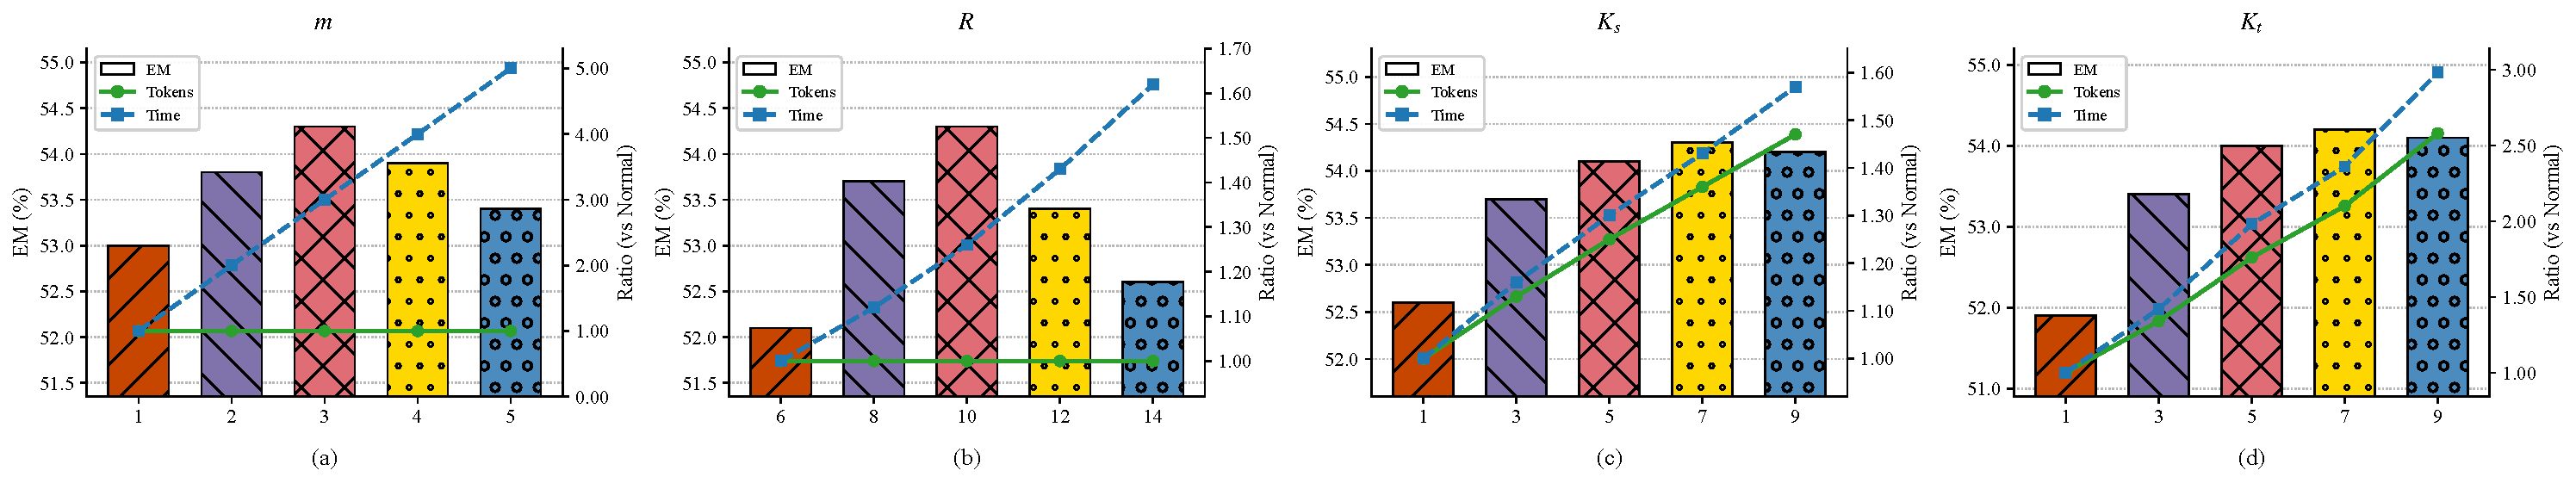
\includegraphics[width=1.0\linewidth]{Figs/hyperparam_2x2_final.pdf}
   \caption{Hyperparameter sensitivity on HotpotQA with KGs constructed by GPT-4o-mini. We vary (a) the number of relation variants $m$, (b) the relation-aligned candidate budget $R$, (c) the structural candidate budget $K_s$, and (d) the textual recovery budget $K_t$, and report EM, normalized retrieval time, and normalized inference tokens.}
    \label{fig:hparam}
\end{figure*}

Figure~\ref{fig:hparam} reports the results of $m$, $R$, $K_s$, and $K_t$ on HotpotQA with KGs constructed by GPT-4o-mini, where online retrieval time and inference tokens are normalized by the smallest setting of each hyperparameter. The results show a common accuracy-efficiency trade-off across these hyperparameters, but they affect different parts of the pipeline. 
For $m$, moderate values perform better because too few relation variants may miss valid structural matches, while too many expand the matching space and introduce loosely related candidates. The $R$ follows a related accuracy and efficiency pattern, where increasing the relation-aligned candidate budget lowers EM while increasing retrieval time, suggesting that retaining more candidates before reranking can introduce additional compatible but irrelevant candidates into contextual reranking. 
For both $m$ and $R$, the token ratio remains unchanged because they affect candidate search and reranking before final evidence packing, rather than changing the number of evidence items fed into the final QA model. For $K_s$, preserving more structural candidates improves EM at first, but the gain quickly saturates once the main constraint-compatible evidence is covered. For $K_t$, larger textual recovery budgets increase the token ratio more clearly, since recovered passages are directly included in the final QA model. 
These trends suggest that the parameters in both retrieval and recovery should be set to moderate values, as larger budgets mainly increase online overhead after the useful evidence has been covered.

\subsection{Constraint Statistics}
\label{appsec:decomp_stats}

We summarize constraint statistics to examine whether CS-RAG represents multi-hop queries through explicit variable dependencies rather than shallow one-hop expansions.
For each dataset, we report full-query statistics, including the average numbers of atomic constraints and variables, as well as the proportions of one-variable and two-variable constraints.
Table~\ref{tab:decomp_stats} shows the results across datasets.
MuSiQue has the largest average number of constraints, reflecting its more compositional query structure and the need to organize reasoning into longer constraint chains.
Its average number of variables is also high, indicating that these chains often involve intermediate entities that must be grounded across hops.
2Wiki has fewer constraints on average, but its average number of variables is comparable to MuSiQue and even slightly higher. This suggests that 2Wiki queries tend to form more compact but variable-dense constraint plans, where multiple entities or values must be resolved within a shorter reasoning structure.
In contrast, HotpotQA has a lower average number of variables and a higher proportion of one-variable constraints, suggesting that more constraints can be directly executed from observed anchors, with fewer variable-variable dependencies.
We also observe a small number of constraints whose head and tail are both observed entities.
For these cases, we try to perform direct textual retrieval and use the retrieved evidence as auxiliary support. However, their impact on the final results is negligible, because most of them simply restate query conditions rather than introduce new binding targets.
\begin{table*}[h]
\centering
\caption{Constraint statistics across three datasets.}
\label{tab:decomp_stats}
\resizebox{0.8\textwidth}{!}{
\begin{tabular}{lccccc}
\toprule
\textbf{Dataset} & \textbf{Avg. Constraints} & \textbf{Avg. Variables} & \textbf{One-Variable (\%)} & \textbf{Two-Variable (\%)}  \\
\midrule
MuSiQue          & 2.89 & 2.32 & 57.08 & 40.23  \\
2Wiki  & 2.41 & 2.35 & 60.95 & 38.59  \\
HotpotQA         & 2.49 & 1.65 & 70.24 & 27.78  \\
\bottomrule
\end{tabular}
}
\end{table*}


\subsection{Correctness of the Sufficiency Check}
\label{app:sufficiency_correctness}
%% musique 2.5 50%  31.9  44.9

To validate that the sufficiency check provides a meaningful confidence signal rather than an arbitrary threshold heuristic, we analyze its behavior under KGs constructed by different builders.
For each dataset, we randomly sample 200 validation queries and run CS-RAG on the KGs constructed by different builders.
We use the same trade-off thresholds as in the main experiments, with \(\gamma=1.5\) for MuSiQue, \(\gamma=1.6\) for 2Wiki, and \(\gamma=2.0\) for HotpotQA, and keep the threshold fixed across builders within the same dataset.
For each executed constraint hop, we record whether it is resolved and whether the induced binding matches the bridge entity or value implied by the gold supporting evidence.
We report Res. as the rate of resolved structural hops and B-Prec. as the binding accuracy among resolved hops.

Table~\ref{tab:builder_sufficiency} shows that stronger builders allow more constraint hops to pass the sufficiency check, indicating that their KGs more often provide concentrated structural evidence.
For weaker builders, Res. decreases substantially, showing that the check filters a larger fraction of uncertain structural candidates before they can be propagated.
Despite this variation in Res., B-Prec. remains consistently high across builders and datasets, indicating that the accepted structural bindings are generally reliable.
This behavior supports the role of $N_{\mathrm{eff}}$ as a confidence signal for structural propagation.



\begin{table*}[h]
\centering
\caption{Resolved-hop rates and binding precision across KG builders on three datasets.}
\label{tab:builder_sufficiency}
\resizebox{0.85\textwidth}{!}{
\begin{tabular}{lcccccc}
\toprule
\multirow{2}{*}{KG Builder} 
& \multicolumn{2}{c}{MuSiQue} 
& \multicolumn{2}{c}{2Wiki} 
& \multicolumn{2}{c}{HotpotQA} \\
\cmidrule(lr){2-3} \cmidrule(lr){4-5} \cmidrule(lr){6-7}
& Res. (\%) & B-Prec. (\%) 
& Res. (\%) & B-Prec. (\%) 
& Res. (\%) & B-Prec. (\%) \\
\midrule
Qwen-3-1.7B   & 13.8 & 91.4 & 18.4 & 95.2 & 15.6 & 88.8 \\
Qwen-3-14B    & 26.5 & 87.6 & 32.7 & 92.4 & 38.9 & 86.5 \\
Llama-3.1-70B & 30.4 & 84.8 & 38.3 & 90.7 & 52.7 & 87.8 \\
GPT-4o-mini   & 44.9 & 88.0 & 45.8 & 93.6 & 61.5 & 90.3 \\
Gemini-2.5-flash-lite   & 46.9 & 82.5 & 42.9 & 87.4 & 60.4 & 91.3 \\
\bottomrule
\end{tabular}
}
\end{table*}


% \begin{table*}[h]
% \centering
% \small
% \setlength{\tabcolsep}{4.5pt}
% \caption{Correctness of sufficiency check across datasets.}

% \begin{tabular}{c cccc cccc cccc}
% \toprule
%  & \multicolumn{4}{c}{MuSiQue} & \multicolumn{4}{c}{2Wiki} & \multicolumn{4}{c}{HotpotQA} \\
% \cmidrule(lr){2-5}\cmidrule(lr){6-9}\cmidrule(lr){10-13}
% $\gamma$ & Rate & Res & Prec & Conf-W & Rate & Res & Prec & Conf-W & Rate  & Res & Prec & Conf-W \\
% \midrule
% 0.5 & & 15.6 & 93.0 & 1.1 & & 24.2 & 96.2 & 0.9 & & 20.4 & 92.1 & 1.6 \\
% 1.0 & & 34.9 & 88.5 & 4.0 & & 48.6 & 92.7 & 3.5 & & 44.1 & 89.2 & 4.8 \\
% 1.5 & & 52.7 & 83.0 & 9.0 & & 66.8 & 89.6 & 6.9 & & 61.5 & 86.3 & 8.4 \\
% 2.0 & & 69.8 & 75.6 & 17.0 & & 79.1 & 84.2 & 12.5 & & 74.6 & 80.0 & 14.9 \\
% 2.5 & & 80.9 & 70.4 & 24.0 & & 86.7 & 79.0 & 18.2 & & 83.4 & 74.8 & 21.0 \\
% \bottomrule
% \end{tabular}

% \label{tab:gating_correctness_all}
% \end{table*}

\subsection{Efficiency Analysis}
\label{appsec:efficiency}

We further evaluate the online retrieval efficiency of CS-RAG under GPT-4o-mini constructed KGs.
Table~\ref{tab:efficiency_all} reports average retrieval latency, retrieval-time LLM token cost, and QA performance on three datasets, excluding offline KG construction and final answer generation. 
Graph-based baselines such as LightRAG, HippoRAG2, and GFM-RAG avoid retrieval-time LLM calls and therefore have zero Token overhead.
NeuroPath incurs higher latency and token usage due to online path-level semantic control.
CS-RAG introduces only a lightweight one-shot planning cost, while avoiding repeated LLM-guided retrieval rounds.
These results show that CS-RAG improves robustness without introducing excessive online retrieval overhead.
\begin{table*}[h]
\centering
\scriptsize
\setlength{\tabcolsep}{3.2pt}
\caption{Efficiency comparison on MuSiQue, 2Wiki, and HotpotQA under GPT-4o-mini constructed KGs.
Time denotes average online retrieval latency in seconds per example and Token denotes the LLM token cost incurred during online retrieval. CS-RAG uses the same trade-off hyperparameters as the main experiments.}
\label{tab:efficiency_all}
\resizebox{1.0\textwidth}{!}{
\begin{tabular}{lcccccccccccc}
\toprule
\multirow{2}{*}{\textbf{Method}} 
& \multicolumn{4}{c}{\textbf{MuSiQue}} 
& \multicolumn{4}{c}{\textbf{2WikiMultihopQA}} 
& \multicolumn{4}{c}{\textbf{HotpotQA}} \\
\cmidrule(lr){2-5} \cmidrule(lr){6-9} \cmidrule(lr){10-13}
& \textbf{Time (S)} & \textbf{Token} & \textbf{EM (\%)} & \textbf{F1 (\%)}
& \textbf{Time (S)} & \textbf{Token} & \textbf{EM (\%)} & \textbf{F1 (\%)}
& \textbf{Time (S)} & \textbf{Token} & \textbf{EM (\%)} & \textbf{F1 (\%)} \\
\midrule
LightRAG   & 1.8 & 0.0  & 3.1  & 9.7  & 1.2 & 0.0  & 9.8  & 18.4 & 1.4 & 0.0  & 15.2 & 26.9 \\
HippoRAG2  & 3.2 & 0.0  & 30.6 & 42.2 & 1.9 & 0.0  & 51.5 & 60.3 & 2.5 & 0.0  & 50.7 & 64.7 \\
GFM-RAG    & 2.8 & 0.0  & 30.5 & 40.9 & 1.6 & 0.0  & 67.8 & 76.9 & 2.0 & 0.0  & 51.2 & 68.0 \\
NeuroPath  & 7.3 & 2.6k & 31.2 & 43.5 & 5.8 & 2.0k & 63.4 & 73.2 & 6.7 & 2.2k & 51.5 & 64.9 \\
\midrule
\textbf{CS-RAG} 
           & 6.3 & 0.86k & 32.2 & 45.1 & 1.7 & 0.72k & 63.0 & 71.0 & 2.2 & 0.76k & 54.3 & 69.8 \\
\bottomrule
\end{tabular}
}
\end{table*}

\subsection{Planner Error Statistics}
\label{app:planner_error_stats}

We evaluate planner output quality to verify that the atomic constraint planning step provides a reliable basis for constraint-based retrieval, rather than introducing frequent planning errors.
Since planner quality directly affects whether retrieval can be grounded in valid constraints, a sufficiently reliable planner is a prerequisite for effective constraint-based retrieval.
For each dataset, we randomly sample 200 queries, generate atomic constraints with the GPT-4o-mini planner, and manually inspect whether each generated constraint correctly reflects the intended reasoning step of the original query, focusing on two aspects: relation semantics and variable usage.
A constraint is marked as incorrect if its relation meaning is drifted or misaligned, or if its variable is missing, swapped, or inconsistently reused.

We report two statistics.
Hop-error rate is the fraction of incorrect constraints among all generated constraints.
Plan-invalid rate is the fraction of queries whose generated plan contains at least one incorrect constraint.
Table~\ref{tab:planner_error_stats} shows that planner errors are relatively infrequent across datasets.
MuSiQue has a slightly higher error rate, which is consistent with its longer and more compositional query structure.
The overall low error rates indicate that the current LLM-based planner provides sufficient planning quality for constructing effective retrieval constraints, making CS-RAG less affected by planner-side errors in our experiments.

\begin{table}[h]
\centering
\small
\setlength{\tabcolsep}{8pt}
\caption{Planner error statistics on 200 sampled queries per dataset.}
\begin{tabular}{l ccc}
\toprule
Metric (\%) & MuSiQue & 2Wiki & HotpotQA \\
\midrule
Hop-error rate $\downarrow$ & 4.6 & 2.8 & 3.4 \\
Plan-invalid rate $\downarrow$            & 7.5 & 4.0 & 5.5 \\
\bottomrule
\end{tabular}

\label{tab:planner_error_stats}
\end{table}


\subsection{Failure Analysis}
\label{app:failure_analysis}

We analyze representative incorrect cases.
Figure~\ref{fig:failure_planner} shows a planner-side error, where the generated constraint plan omits the intermediate variable required by the query and therefore directs retrieval to the wrong entity.
Figure~\ref{fig:failure_evidence} shows an evidence-side insufficiency case, where CS-RAG does not propagate the under-supported binding, but the required bridge evidence is absent or too implicit in both the KG and the recovered textual pool.

\begin{figure*}[h]
\centering
\fbox{
\parbox{0.97\textwidth}{
\footnotesize

\textbf{Query.}
What are the two categories of the non-electric version of the neighbourhood electric vehicle?

\vspace{0.6em}
\fbox{\parbox{0.94\textwidth}{
\textbf{Block 0: Gold evidence chain.}\\[-0.2em]
The query first needs to identify the non-electric version of the neighbourhood electric vehicle, and then retrieve the two categories of that vehicle type.\\
$\tau_0$: neighbourhood electric vehicle \;--\; non-electric version \;--\; ?vehicle\\
$\tau_1$: ?vehicle \;--\; has category \;--\; ?category1\\
$\tau_2$: ?vehicle \;--\; has category \;--\; ?category2\\
\textit{Gold intermediate:} ?vehicle = Motorised quadricycle.\\
\textit{Gold answer:} light quadricycles (L6e) and heavy quadricycles (L7e).
}}

\vspace{0.6em}
\fbox{\parbox{0.94\textwidth}{
\textbf{Block 1: Atomic constraint plan comparison.}\\[-0.2em]
\textit{Expected atomic constraints:}\\
$\tau_0$: neighbourhood electric vehicle \;--\; non-electric version \;--\; ?vehicle\\
$\tau_1$: ?vehicle \;--\; has category \;--\; ?category1\\
$\tau_2$: ?vehicle \;--\; has category \;--\; ?category2\\[0.3em]

\textit{Observed erroneous constraints:}\\
$\tau_0'$: neighbourhood electric vehicle \;--\; has category \;--\; ?category1\\
$\tau_1'$: neighbourhood electric vehicle \;--\; has category \;--\; ?category2\\[0.3em]

\textit{Planner error:} The planner omits the bridge variable ?vehicle required by the phrase ``the non-electric version of the neighbourhood electric vehicle.'' 
Instead of first binding ?vehicle to \emph{Motorised quadricycle}, it directly queries the categories of \emph{neighbourhood electric vehicle}. 
As a result, the generated plan changes the retrieval target from ``categories of Motorised quadricycle'' to ``categories of neighbourhood electric vehicle''.
}}

\vspace{0.6em}
\fbox{\parbox{0.94\textwidth}{
\textbf{Block 2: Retrieval consequence under the wrong executable frontier.}\\[-0.2em]
Because the planner omits the bridge constraint, CS-RAG directly executes the following two constraints:
\[
\tau_0': \text{neighbourhood electric vehicle} \;--\; \text{has category}\;--\; ?\text{category1},
\]
\[
\tau_1': \text{neighbourhood electric vehicle} \;--\; \text{has category}\;--\; ?\text{category2}.
\]
Thus, the retrieval frontier is anchored on \emph{neighbourhood electric vehicle}, rather than on the intended intermediate entity \emph{Motorised quadricycle}. 
Since the local candidate pool around \emph{neighbourhood electric vehicle} contains several classification-like relations, the retriever selects candidates that appear consistent with the erroneous constraints.\\[0.3em]

\textit{Retrieved candidates under the erroneous plan:}\\
(1) neighbourhood electric vehicle \;--\; classified as \;--\; low-speed vehicle\\
(2) neighbourhood electric vehicle \;--\; type of \;--\; battery electric vehicle\\
(3) neighbourhood electric vehicle \;--\; has top speed \;--\; 25 mph\\
(4) neighbourhood electric vehicle \;--\; has maximum loaded weight \;--\; 3,000 lb\\[0.3em]

\textit{Selected bindings under the erroneous plan:}\\
?category1 = low-speed vehicle\\
?category2 = battery electric vehicle\\[0.3em]

\textit{Required but missed bridge and target facts:}\\
neighbourhood electric vehicle \;--\; non-electric version \;--\; Motorised quadricycle\\
Motorised quadricycle \;--\; has category \;--\; light quadricycles (L6e)\\
Motorised quadricycle \;--\; has category \;--\; heavy quadricycles (L7e)\\[0.3em]

\textit{Decision:} The system resolves the two generated category constraints with locally plausible but target-misaligned bindings. 
The final retrieved evidence therefore supports categories of \emph{neighbourhood electric vehicle}, while the gold answer requires categories of its non-electric version, \emph{Motorised quadricycle}.
}}

\vspace{0.6em}
\fbox{\parbox{0.94\textwidth}{
\textbf{Failure diagnosis.}\\[-0.2em]
The failure occurs before structural retrieval begins. 
The planner drops the intermediate bridge variable needed to resolve the phrase ``non-electric version.'' 
CS-RAG then follows the generated constraints and searches for categories of the wrong entity. 
This case therefore reflects a planner-side failure, specifically a missing bridge variable, rather than a failure of constraint-based retrieval or sufficiency checking.
}}

}
}

\caption{Failure analysis of a planner-side error case.}
\label{fig:failure_planner}
\end{figure*}

\begin{figure*}[h]
\centering
\fbox{
\parbox{0.97\textwidth}{
\footnotesize

\textbf{Query.}
When was Lady Godiva's birthplace abolished?

\vspace{0.6em}
\fbox{\parbox{0.94\textwidth}{
\textbf{Block 0: Intended reasoning chain.}\\[-0.2em]
The query requires first identifying Lady Godiva's birthplace, and then retrieving when that place was abolished.\\
$\tau_0$: Lady Godiva \;--\; place of birth \;--\; ?place\\
$\tau_1$: ?place \;--\; abolished in \;--\; ?year\\
\textit{Gold intermediate:} ?place = Mercia.\\
\textit{Gold answer:} ?year = 918.
}}

\vspace{0.6em}
\fbox{\parbox{0.94\textwidth}{
\textbf{Block 1: Structural retrieval for $\tau_0$.}\\[-0.2em]
The structural retriever searches for a birthplace bridge from \emph{Lady Godiva}. 
However, the available KG evidence mainly contains related facts around Godiva, Leofric, and Mercia, rather than a direct birthplace relation.\\[0.3em]
\textit{Retrieved structural candidates:}\\
(1) Lady Godiva \;--\; wife of \;--\; Leofric\\
(2) Spalding Priory \;--\; founded by \;--\; Leofric and Godiva\\
(3) Lady Godiva \;--\; title \;--\; Countess of Leicester\\[0.3em]
\textit{After relation-aware filtering:}\\
(1) Lady Godiva \;--\; wife of \;--\; Leofric\\
(2) Lady Godiva \;--\; title \;--\; Countess of Leicester\\[0.3em]
\textit{Sufficiency signal:} No candidate directly supports the constraint \emph{place of birth}.\\
\textit{Decision:} Unresolved. Do not bind ?place to Mercia.
}}

\vspace{0.6em}
\fbox{\parbox{0.94\textwidth}{
\textbf{Block 2: Textual recovery for $\tau_0$.}\\[-0.2em]
CS-RAG activates textual recovery because the structural hop is unresolved. 
The recovered text still does not provide an explicit bridge from Lady Godiva to Mercia as her birthplace.\\[0.3em]
\textit{Retrieved sentences:}\\
(1) ``It was founded as a cell of Croyland Abbey, in 1052, by Leofric, Earl of Mercia and his wife, Godiva, Countess of Leicester.''\\
(2) ``When \AE thelfl\ae d died in 918, \AE lfwynn, her daughter by \AE thelred, succeeded as Second Lady of the Mercians.''\\
(3) ``Within six months Edward had deprived her of all authority in Mercia and taken her into Wessex.''\\[0.3em]
\textit{Recovery observation:} The retrieved sentences mention Godiva, Leofric, and Mercia, but they do not explicitly state that Lady Godiva's birthplace is Mercia.\\
\textit{Decision:} Still unresolved. The subsequent hop cannot be safely executed.
}}

\vspace{0.6em}
\fbox{\parbox{0.94\textwidth}{
\textbf{Block 3: Failure diagnosis.}\\[-0.2em]
CS-RAG correctly avoids propagating an under-supported binding from Lady Godiva to other entities in Block 1.
This prevents a hallucinated structural chain because the available KG evidence only provides related facts rather than a reliable birthplace bridge.
The failure occurs because textual recovery also fails to retrieve an explicit sentence supporting the missing bridge.
Therefore, the final answer remains unsupported even though the sufficiency check behaves as intended.
This case reflects that CS-RAG can block unsafe continuation, but it cannot recover an answer when the necessary bridge is absent or too implicit in all accessible evidence.
}}

}
}

\caption{Failure analysis of an evidence-side insufficiency case.}
\label{fig:failure_evidence}
\end{figure*}


\subsection{Case Study}

Figure~\ref{fig:case_study_trace} shows a two-hop example illustrating how CS-RAG addresses both spurious noise and incomplete information in an imperfect KG.
The planner converts the query into two atomic constraints with unknown variables (?prison, ?year).
At Hop-1, the 1-hop neighborhood around the anchor contains several semantically similar but constraint-violating tuples, which reflect spurious structural distractors.
After constraint-based retrieval with relation-variant alignment, the candidate distribution becomes concentrated and the sufficiency check yields $N_{\text{eff}}<\gamma$, so the hop is marked as Resolved and ?prison is bound to Tower of London.
At Hop-2, although the candidates remain topically related to the resolved entity, the KG does not provide a tuple that satisfies the target constraint used as a prison until, leading to an ambiguous candidate distribution with $N_{\text{eff}}\ge\gamma$ and an Unresolved decision.
CS-RAG then activates textual recovery, retrieves and reranks passages, and recovers the missing evidence needed to resolve ?year as 1952.
Finally, the QA model is prompted with the query and the constraint-aligned evidence for both hops to generate the answer.

\begin{figure*}[h]
\centering

\fbox{
\parbox{0.97\textwidth}{
\footnotesize

\textbf{Query.}
What year did the prison where \emph{No Cross, No Crown} was written stop being used as a prison?

\vspace{0.6em}
\fbox{\parbox{0.94\textwidth}{
\textbf{Block 0: Atomic constraint planning (unknowns carried across hops).}\\[-0.2em]
$\tau_0$: No Cross, No Crown \;|\; written during imprisonment in \;|\; ?prison\\
$\tau_1$: ?prison \;|\; used as a prison until \;|\; ?year\\
\textit{Note:} Hop-1 resolves ?prison, then Hop-2 resolves ?year (two unknowns solved sequentially).
}}

\vspace{0.6em}
\fbox{\parbox{0.94\textwidth}{
\textbf{Block 1 (Hop-1): solve ?prison from $\tau_0$.}\\[-0.2em]

\textit{Initial 1-hop top-$K$ (before rerank):}\\
(1) No Cross, No Crown \;|\; written during imprisonment in \;|\; Tower of London\\
(2) No Cross, No Crown \;|\; written in \;|\; London\\
(3) No Cross, No Crown \;|\; related to \;|\; Tower Bridge\\
(4) No Cross, No Crown \;|\; composed during incarceration in \;|\; Tower Hamlets\\

\textit{After constraint anchoring + relation-variant rerank:}\\
(1) No Cross, No Crown \;|\; written during imprisonment in \;|\; Tower of London\\
(2) No Cross, No Crown \;|\; written in \;|\; London\\
\textit{Prob. weight:} [0.82, 0.18] \quad \textit{N\_eff:} 1.42 \;(\(< \gamma=2.0\))\\

\textit{Decision:} \textbf{Resolved}. Bind ?prison = Tower of London.
}}

\vspace{0.6em}
\fbox{\parbox{0.94\textwidth}{
\textbf{Block 2 (Hop-2): solve ?year from $\tau_1$.}\\[-0.2em]

\textit{Initial 1-hop top-$K$ (before rerank):}\\
(1) Tower of London \;|\; built in \;|\; 1078\\
(2) Tower of London \;|\; served as \;|\; royal residence\\
(3) Tower of London \;|\; location \;|\; London\\
(4) Tower of London \;|\; attracts \;|\; tourists\\
(5) Tower of London \;|\; held prisoners \;|\; Ranulf Flambard\\
(6) Tower of London \;|\; used for imprisonment during \;|\; Middle Ages\\

\textit{After constraint anchoring + relation-variant rerank:}\\
(1) Tower of London \;|\; built in \;|\; 1078\\
(2) Tower of London \;|\; served as \;|\; royal residence\\
(3) Tower of London \;|\; used for imprisonment during \;|\; Middle Ages\\
\textit{Prob. weight:} [0.25, 0.33, 0.42] \quad \textit{N\_eff:} 2.87 \;(\(\ge \gamma=2.0\))\\

\textit{Decision:} \textbf{Unresolved}.
}}

\vspace{0.6em}
\fbox{\parbox{0.94\textwidth}{
\textbf{Block 3: Textual recovery for $\tau_1$.}\\[-0.2em]

\textit{Retrieved sentences:}\\
(1) ``The castle was used as a prison \dots\ until 1952.''\\
(2) ``A grand palace early in its history, it served as a royal residence \dots''\\
(3) ``The White Tower was built in 1078 \dots''\\

Recovery result: textual evidence supports the answer 1952 without propagating a structural binding.
% \textit{Decision:} \textbf{Resolved}. Bind ?year = 1952.
}}

} % end parbox
} % end fbox

\caption{A case study trace for \textsc{CS-RAG} (two-hop). Each block reports initial 1-hop top-$K$ candidates (before rerank), the constraint-aware reranked distribution, the solvability signal (N\_eff vs. threshold \(\gamma\)), and the hop decision (Resolved / Unresolved) with optional textual recovery and final answer generation.}
\label{fig:case_study_trace}
\end{figure*}


%%%%QA:
\section{LLM Prompt}

Figure~\ref{fig:prompt_query_decomposition} shows the prompt used for atomic constraint planning, which converts the original query into a minimal multi-hop chain of query triples with relation variants for downstream structural retrieval.
Figure~\ref{fig:prompt_example} shows the reasoning prompt used for hop-wise evidence reasoning, where the model is provided with atomic constraints and their retrieved evidence blocks and is required to output only the final short answer.

\begin{figure*}[ht]
    \centering
    \setstretch{1.0}
    \begin{fullwidthprompt}
You are an expert in Knowledge Graphs and Query Answering. 
Your task is to perform constraint planning by converting a complex natural language query into an ordered sequence of atomic constraints. Use the following rules:

\vspace{0.3em}
\begin{itemize}
    \setlength\itemsep{0em}
    \item Identify known entities and use \texttt{?}-prefixed variables for unknown ones.
    \item Reuse the same variable only when it clearly refers to the same unknown.
    \item Output a valid JSON object with one key: \texttt{"triples"}.
    \item Each element in \texttt{"triples"} must be an object containing:
    \begin{itemize}
        \setlength\itemsep{0em}
        \item \texttt{"head"}: string
        \item \texttt{"relation"}: string
        \item \texttt{"relation\_variants"}: m short, logically similar relation strings
        \item \texttt{"tail"}: string
    \end{itemize}
    \item Triples must form a minimal yet sufficient reasoning chain: filling all \texttt{?} enables answering the query using only these triples.
    \item For property queries (nationality/position/time/location/etc.), link the property \texttt{?} directly to the target entity variable, not a side entity.
    \item Make \texttt{"relation\_variants"} informative enough to be understood without the original query.
    \item Encode extra conditions on the same entity variable, or merge them into the entity mention as modifiers; do not drop useful descriptors.
    \item Never let one variable represent multiple distinct unknowns; use separate names when unclear. (e.g. \texttt{?country1}, \texttt{?country2}) when needed.
    \item If the query provides a concrete value (country/year/location), connect directly to it; don't introduce a \texttt{?} just to equal that value.
    \item Keep variable names short/generic; express details via relations/triples, not long variable names.
    \item Prefer triples that contain at least one ?-variable; avoid known-known triples unless they are necessary to preserve an explicit query condition.
\end{itemize}

\vspace{0.3em}
Examples:
\vspace{0.3em}

\textbf{Query}: ``When did Lothair II's mother die?''\\
\textbf{Output}:{\footnotesize
\begin{verbatim}
{
  "triples": [
    {
      "head": "Lothair II",
      "relation": "has mother",
      "relation variants": [ "has parent", "mother is", "is child of"],
      "tail": "?person"
    },
    {
      "head": "?person",
      "relation": "died on",
      "relation variants": ["date of death", "passed away on", "death date"],
      "tail": "?date"
    }
  ]
}
\end{verbatim}
}
\textbf{Query:}
    \end{fullwidthprompt}
    \caption{The prompt used for atomic constraint planning.}
    \label{fig:prompt_query_decomposition}
\end{figure*}


\begin{figure*}[ht]
    \centering
    
    \setstretch{1.15}
    \begin{fullwidthprompt}
You are a strict multi hop inference assistant that can complete multi hop inference based on given information.
Now, you need to conduct rigorous and rational multi-step thinking based on the given search evidence to answer this query. You only need to use the given information to answer the query.
We perform Atomic Constraint Planning and obtain multiple atomic constraints. For each atomic constraint, several pieces of relevant evidence are retrieved. You should use the provided evidence to resolve the variables in the atomic constraints step by step, and derive the final answer.
You can only answer the final answer with short and appropriate phrases (such as names, numbers, or short noun phrases that conform to the query format). Do not include explanations, sentences, or any other words.
Here is the information you can obtain:

Query: How many times did the plague occur in the city where the painter of The Bacchanal of the Andrians died?

The atomic constraint plan is as follows. Each atomic constraint contains an approximate relation expression and a variable that should be resolved using the retrieved evidence. For each atomic constraint, the retrieved evidence is provided below:

$\tau_0$: The Bacchanal of the Andrians | painted by | ?painter
  
     
     Evidence 1: $<$ retrieved evidence text $>$ 
     
    Evidence 2: $<$ retrieved evidence text $>$ 
    
    Evidence 3: $<$ retrieved evidence text $>$  

$\tau_1$: ?painter | died in | ?city
 
    
    Evidence 1: $<$ retrieved evidence text $>$ 
    
        Evidence 2: $<$ retrieved evidence text $>$  
        
    Evidence 3: $<$ retrieved evidence text $>$  

$\tau_2$: ?city | number of plague occurrences | ?count
 
    
    Evidence 1: $<$ retrieved evidence text $>$ 
    
        Evidence 2: $<$ retrieved evidence text $>$  
        
    Evidence 3: $<$ retrieved evidence text $>$  
    

Based on the above information, answer the query.

Query: How many times did the plague occur in the city where the painter of The Bacchanal of the Andrians died? Answer:
    \end{fullwidthprompt}
    \caption{A QA prompt template of CS-RAG used for multi-hop reasoning.}
    \label{fig:prompt_example}
\end{figure*}




%%%%%%%%%%%%%%%%%%%%%%%%%%%%%%%%%%%%%%%%%%%%%%%%%%%%%%%%%%%%%%%%%%%%%%%%%%%%%%%
%%%%%%%%%%%%%%%%%%%%%%%%%%%%%%%%%%%%%%%%%%%%%%%%%%%%%%%%%%%%%%%%%%%%%%%%%%%%%%%

\end{document}
